% ==========================================
% PHỤ LỤC A: PHÂN TÍCH CHUYÊN SÂU KIẾN TRÚC VÀ TÍNH KHẢ THI TRÊN ĐA DẠNG DỮ LIỆU
% ==========================================
\chapter{PHÂN TÍCH CHUYÊN SÂU KIẾN TRÚC VÀ TÍNH KHẢ THI TRÊN ĐA DẠNG DỮ LIỆU}
\label{AppendixA}

Phụ lục A tập hợp các số liệu chi tiết mà Chương~\ref{Chapter4} chỉ nhắc ngắn gọn: chi phí tính toán, nghiên cứu loại bỏ thành phần, độ ổn định khi chia lại dữ liệu nhiều lần, và hiệu năng theo từng nhóm đặc tính tổn thương trên cả BTXRD (Mục~\ref{subsec:arch_btxrd}) lẫn FracAtlas (Mục~\ref{subsec:arch_fracatlas}). Việc tách riêng phần này giúp Chương~\ref{Chapter4} tập trung vào các nhận định chính, đồng thời thuận tiện cho việc tra cứu và đối chiếu các số liệu thực nghiệm chi tiết.

% ------------------------------------------------------------
\section{Hiệu quả tính toán của PGA-UNet và SAM-Med2D}
\label{sec:appendix_efficiency}
% ------------------------------------------------------------

Mục này trình bày đầy đủ số liệu của phần đo hiệu quả tính toán đã được tóm tắt ở Chương~\ref{Chapter4}. Các phép đo được thực hiện trong cùng môi trường chạy, với cùng thiết bị và cùng cách đo cho từng mô hình. Những chỉ số được ghi nhận gồm số tham số, số tham số có thể huấn luyện, số phép tính, dung lượng checkpoint, bộ nhớ GPU đỉnh và độ trễ suy luận trung bình trên GPU và CPU. SAM-Med2D được đo ở $256\times256$, còn PGA-UNet được đo ở hai cấu hình $256\times256$ và $512\times512$ để tiện đối sánh trực tiếp. Các con số trong mục này chỉ được hiểu là để so sánh tương đối trong cùng môi trường thực nghiệm.

\begin{table}[H]
    \centering
    \caption{Bảng so sánh hiệu quả tính toán giữa PGA-UNet và SAM-Med2D trong cùng môi trường thực nghiệm}
    \label{tab:appendix_efficiency_comparison}
    \renewcommand{\arraystretch}{1.3}
    \resizebox{\textwidth}{!}{%
    \begin{tabular}{|l|c|c|c|c|c|c|c|}
        \hline
        \textbf{Mô hình}
        & \textbf{Tham số tổng (M)}
        & \textbf{Tham số học (M)}
        & \textbf{FLOPs (G)}
        & \textbf{Checkpoint (MB)}
        & \textbf{Bộ nhớ GPU đỉnh (MB)}
        & \textbf{Độ trễ GPU (ms/ảnh)}
        & \textbf{Độ trễ CPU (ms/ảnh)} \\
        \hline
        PGA-UNet ($256\times256$) & 2.950 & 2.950 & 7.742 & 11.3 & 3300.8 & 8.46 $\pm$ 0.83 & 83.87 $\pm$ 2.08 \\
        \hline
        PGA-UNet ($512\times512$) & 2.950 & 2.950 & 30.968 & 11.3 & 3429.8 & 21.83 $\pm$ 0.23 & 309.84 $\pm$ 8.24 \\
        \hline
        SAM-Med2D ($256\times256$) & 271.242 & 184.569 & 92.024 & 2443.2 & 3332.8 & 60.70 $\pm$ 1.54 & 769.40 $\pm$ 11.36 \\
        \hline
    \end{tabular}%
    }
\end{table}

Ở cùng độ phân giải $256\times256$, chênh lệch là rất lớn: SAM-Med2D nhiều tham số hơn khoảng 92 lần, số phép tính cao hơn gần 12 lần, checkpoint lớn hơn 215 lần, và chậm hơn PGA-UNet khoảng 7,2 lần trên GPU. Trên CPU khoảng cách này còn lớn hơn khoảng 9,2 lần. Với một hệ thống tương tác trực tiếp, việc phản hồi nhanh hơn sau mỗi thao tác chỉnh câu nhắc sẽ mang lại trải nghiệm tốt hơn so với việc bác sĩ phải chờ đợi mô hình xử lý.

\begin{figure}[H]
    \centering
    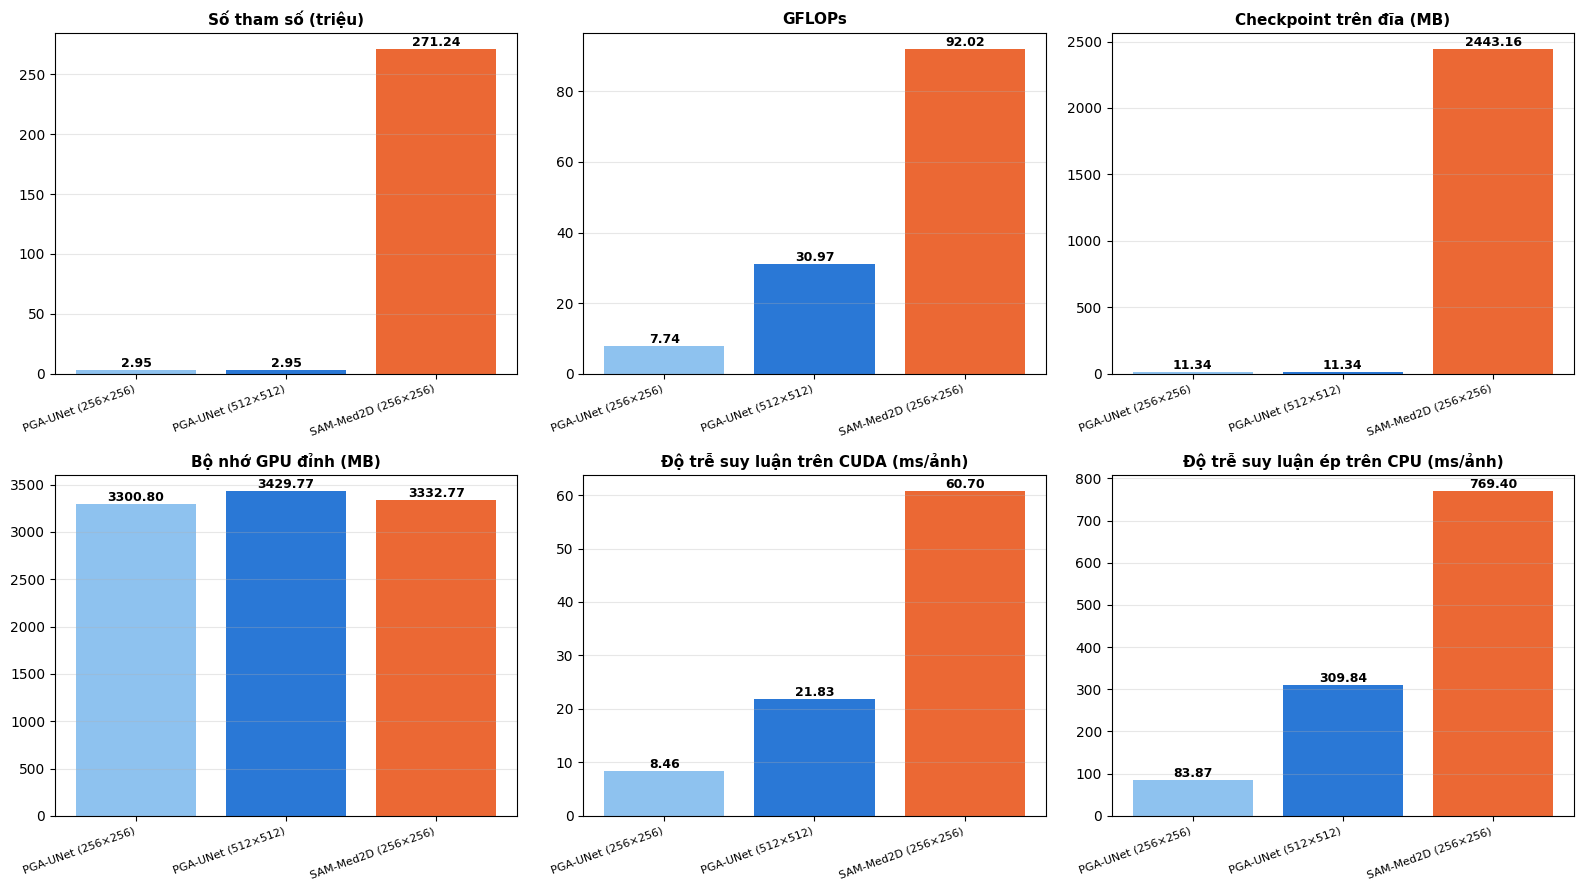
\includegraphics[width=0.95\textwidth]{images/efficiency_comparison_from_notebook.png}
    \caption{Biểu đồ tổng hợp sáu chỉ số hiệu quả tính toán giữa PGA-UNet và SAM-Med2D.}
    \label{fig:appendix_efficiency_comparison}
\end{figure}

Bộ nhớ GPU đỉnh là chỉ số duy nhất chưa cho thấy khoảng cách rõ như các chỉ số còn lại. Khả năng cao là vì chỉ số này còn phụ thuộc cách khung chạy cấp phát bộ nhớ, không chỉ phụ thuộc kiến trúc mô hình. Vì vậy, khi so sánh chi phí triển khai, khóa luận ưu tiên nhìn vào số tham số, số phép tính, dung lượng checkpoint và độ trễ suy luận.

% ------------------------------------------------------------
\section{Phân tích trên BTXRD}
\label{subsec:arch_btxrd}
% ------------------------------------------------------------

Trên BTXRD, PGA-UNet được phân tích theo ba hướng: đóng góp của từng thành phần kiến trúc, độ ổn định qua các lần chia dữ liệu ngẫu nhiên, và hiệu năng theo đặc tính tổn thương. Trong từng nhóm thí nghiệm, các cấu hình đều được đánh giá trên cùng dữ liệu, cùng kịch bản câu nhắc và cùng cách tính chỉ số ở cấp độ ảnh.

\subsection{Đóng góp của kiến trúc và câu nhắc}
\label{subsec:ablation_arch}

\noindent\textbf{Thiết kế thí nghiệm}\\
Tám cấu hình được huấn luyện lại từ đầu trên cùng tập BTXRD và giữ nguyên các điều kiện huấn luyện. Thực nghiệm chỉ thay đổi ba yếu tố: PSG tại bộ mã hóa, cơ chế chú ý trên các kết nối tắt của nhánh giải mã và cách biểu diễn câu nhắc.

Trong đó, sáu cấu hình cùng sử dụng bản đồ nhiệt Gaussian để khảo sát đóng góp kiến trúc. Mỗi cấu hình là một tổ hợp giữa hai lựa chọn tại bộ mã hóa (không hoặc có PSG) và ba lựa chọn cho cơ chế chú ý trên các kết nối tắt của nhánh giải mã (không dùng cổng chú ý, dùng cổng chú ý nguyên bản hoặc dùng CAD). Nhờ đó, xác định PSG và CAD có hiệu quả khi hoạt động riêng lẻ hay chỉ phát huy khi được kết hợp.

Hai cấu hình còn lại thay bản đồ nhiệt Gaussian bằng mặt nạ hộp giới hạn nhị phân. Chúng được dùng để so sánh hai cách biểu diễn câu nhắc trong cả cấu hình nối kênh cơ sở và cấu hình đầy đủ PSG+CAD.

U-Net+Concat là cấu hình cơ sở, trong đó câu nhắc chỉ được nối vào ảnh như một kênh đầu vào. U-Net+PSG và U-Net+CAD lần lượt bổ sung riêng PSG hoặc CAD. Các cấu hình dùng cổng chú ý nguyên bản kế thừa Attention U-Net~\cite{oktay2018attentionunet} và không nhận trực tiếp đặc trưng câu nhắc trong cơ chế chú ý trên các kết nối tắt của nhánh giải mã. PGA-UNet kết hợp cả PSG, CAD và bản đồ nhiệt Gaussian.

\begin{table}[H]
    \centering
    \caption{Kết quả chỉ số Dice của nghiên cứu loại bỏ thành phần trên BTXRD trong ba kịch bản câu nhắc (N=\Ntestimg~ảnh)}
    \label{tab:ablation_arch}
    \renewcommand{\arraystretch}{1.3}
    \resizebox{\textwidth}{!}{%
    \begin{tabular}{|l|c|c|c|c|c|c|}
        \hline
        \textbf{Cấu hình}
        & \textbf{PSG}
        & \textbf{Chú ý trên kết nối tắt}
        & \textbf{Câu nhắc}
        & \textbf{Bao trọn↑}
        & \textbf{Lệch tâm↑}
        & \textbf{Hỗn hợp↑} \\
        \hline
        U-Net+Concat (Gaussian)
        & \texttimes & Không & Gaussian
        & 0.8763 & 0.7364 & 0.8216 \\
        \hline
        U-Net+PSG
        & \checkmark & Không & Gaussian
        & 0.8673 & 0.7388 & 0.8162 \\
        \hline
        U-Net+CAD
        & \texttimes & CAD & Gaussian
        & \textbf{0.8861} & 0.7406 & 0.8292 \\
        \hline
        PGA-UNet (nhị phân)
        & \checkmark & CAD & Nhị phân
        & 0.8780 & 0.7434 & 0.8267 \\
        \hline
        U-Net+Concat (nhị phân)
        & \texttimes & Không & Nhị phân
        & 0.8781 & 0.7312 & 0.8202 \\
        \hline
        \textbf{PGA-UNet}
        & \checkmark & CAD & Gaussian
        & 0.8607 & \textbf{0.8423} & \textbf{0.8560} \\
        \hline
        U-Net+PSG+Cổng chú ý nguyên bản
        & \checkmark & Nguyên bản & Gaussian
        & 0.8680 & 0.7359 & 0.8173 \\
        \hline
        U-Net+Cổng chú ý nguyên bản
        & \texttimes & Nguyên bản & Gaussian
        & 0.8738 & 0.7314 & 0.8193 \\
        \hline
    \end{tabular}%
    }
\end{table}

\noindent\textbf{Vai trò của thông tin câu nhắc}\\
Điểm đáng chú ý đầu tiên là lợi ích lớn nhất đến từ việc có câu nhắc. U-Net không dùng câu nhắc chỉ đạt Dice 0,4740 trên BTXRD (Ở bảng~\ref{tab:baseline_comparison}), trong khi cách đơn giản nhất là nối thẳng câu nhắc vào ảnh đầu vào đã nâng Dice lên 0,8763 ở kịch bản Bao trọn. Nghĩa là trước khi xét đến PSG hay CAD, bản thân thông tin câu nhắc đã tạo ra khác biệt rất lớn.

Attention U-Net không có câu nhắc đạt kết quả thấp hơn U-Net không câu nhắc. Kết quả này cho thấy cổng chú ý nguyên bản không tự cải thiện hiệu năng trong thiết lập hiện tại khi thiếu thông tin định hướng. Tuy nhiên, số liệu này không phải là nguyên nhân gây suy giảm mà chỉ được sử dụng làm điểm tham chiếu cho các cấu hình chú ý có câu nhắc.

\noindent\textbf{Đóng góp của PSG tại bộ mã hóa}\\
Khi được sử dụng riêng lẻ, PSG tạo ra mức thay đổi nhỏ so với phép nối kênh. Trong kịch bản Lệch tâm, Dice tăng từ 0,7364 của U-Net+Concat lên 0,7388 của U-Net+PSG, tương ứng mức tăng 0,0024. Ngược lại, Dice giảm nhẹ 0,0090 ở kịch bản Bao trọn và 0,0054 ở kịch bản Hỗn hợp.

Khi xét riêng, PSG chưa đủ để tạo ra cải thiện rõ rệt ở đầu ra phân đoạn. Vai trò chính của PSG không phải là thay thế quá trình tái tạo mặt nạ, mà là đưa tín hiệu không gian của câu nhắc vào quá trình mã hóa đặc trưng. Lợi ích của tín hiệu này chỉ thể hiện rõ hơn khi nhánh giải mã tiếp tục khai thác thông qua CAD trên các kết nối tắt.

\noindent\textbf{Đóng góp của CAD trên các kết nối tắt của nhánh giải mã}\\
Khi không có PSG, U-Net+CAD đạt Dice 0,8861 ở kịch bản Bao trọn, cao nhất trong tám cấu hình. So với U-Net+Concat, CAD cải thiện Dice 0,0098 ở Bao trọn, 0,0042 ở Lệch tâm và 0,0076 ở Hỗn hợp. Như vậy, CAD riêng lẻ giúp cơ chế chú ý trên các kết nối tắt khai thác câu nhắc tốt hơn phép nối kênh, nhưng mức cải thiện trong kịch bản Lệch tâm vẫn còn nhỏ.

Vai trò của việc điều kiện hóa chú ý thể hiện rõ hơn khi so sánh CAD với cổng chú ý nguyên bản. Không có PSG, U-Net+CAD cao hơn U-Net+Cổng chú ý nguyên bản 0,0123 ở Bao trọn, 0,0092 ở Lệch tâm và 0,0099 ở Hỗn hợp. Khi có PSG, PGA-UNet cao hơn U-Net+PSG+Cổng chú ý nguyên bản 0,1064 ở Lệch tâm và 0,0387 ở Hỗn hợp, mặc dù thấp hơn 0,0073 ở Bao trọn. Điều này cho thấy lợi ích chính không đến từ việc bổ sung một cổng chú ý bất kỳ, mà từ việc điều kiện hóa quá trình chú ý bằng đặc trưng câu nhắc thông qua CAD.

\noindent\textbf{Đóng góp của bản đồ nhiệt Gaussian}\\
Ở cấu hình nối kênh cơ sở, cách biểu diễn câu nhắc chỉ tạo ra khác biệt nhỏ. So với U-Net+Concat dùng mặt nạ nhị phân, U-Net+Concat dùng Gaussian thấp hơn 0,0018 ở Bao trọn, nhưng cao hơn 0,0052 ở Lệch tâm và 0,0014 ở Hỗn hợp. Những chênh lệch này đều nhỏ hơn 0,006.

Ảnh hưởng của Gaussian trở nên rõ rệt khi câu nhắc được xử lý bởi đầy đủ PSG và CAD. So với PGA-UNet dùng câu nhắc nhị phân, PGA-UNet dùng Gaussian cao hơn 0,0989 Dice ở kịch bản Lệch tâm và 0,0293 ở Hỗn hợp, nhưng thấp hơn 0,0173 ở Bao trọn. Có thể thấy mặt nạ nhị phân phù hợp hơn một chút khi hộp giới hạn hoàn toàn chính xác, trong khi bản đồ nhiệt Gaussian giúp mô hình duy trì hiệu năng tốt hơn khi vị trí câu nhắc bị lệch trong phạm vi bài toán.

Có thể hiểu rằng sự chuyển tiếp mềm của bản đồ nhiệt Gaussian làm mô hình bớt phụ thuộc vào đường biên cứng của hộp giới hạn. Dù vậy, đây vẫn chỉ là cách giải thích dựa trên thiết kế và kết quả thực nghiệm, chưa phải bằng chứng trực tiếp về cách mô hình tổ chức đặc trưng bên trong.

\noindent\textbf{Sự bổ trợ giữa PSG, CAD và bản đồ nhiệt Gaussian}\\
Trong kịch bản Lệch tâm, PSG riêng lẻ cải thiện 0,0024 và CAD riêng lẻ cải thiện 0,0042 so với U-Net+Concat. Trong khi đó, cấu hình kết hợp PSG, CAD và Gaussian cải thiện 0,1059. Chênh lệch này cho thấy hiệu quả của mô hình không phải là tổng đơn giản của hai thành phần hoạt động độc lập, mà xuất hiện khi tín hiệu câu nhắc được duy trì xuyên suốt cả bộ mã hóa và các kết nối tắt có chú ý của nhánh giải mã.

Theo cơ chế thiết kế, PSG đưa thông tin không gian của câu nhắc vào các đặc trưng mã hóa, CAD sử dụng đặc trưng câu nhắc để điều chỉnh các kết nối tắt của nhánh giải mã, còn bản đồ nhiệt Gaussian cung cấp tín hiệu không gian có chuyển tiếp mềm. Ba thành phần vì vậy đảm nhận các vai trò khác nhau nhưng liên kết trong cùng một quá trình dẫn hướng phân đoạn. Nhận xét này dựa trên chênh lệch Dice trung bình và được xem là bằng chứng về xu hướng bổ trợ, không phải một kiểm định tương tác chính thức.

\noindent\textbf{Kết luận từ nghiên cứu loại bỏ thành phần}\\
Hạn chế của PGA-UNet nằm ở kịch bản Bao trọn, tức là khi câu nhắc gần như lý tưởng. Ở đây PGA-UNet (0,8607) thấp hơn U-Net+CAD (0,8861) một khoảng 0,0254. Điều này phù hợp với đặc điểm thiết kế: mặt nạ nhị phân có biên rõ nên có lợi khi vị trí hộp giới hạn hoàn toàn chính xác, còn bản đồ nhiệt Gaussian chấp nhận giảm nhẹ hiệu năng để đổi lấy độ bền khi câu nhắc bị lệch. Trong thực tế, khi bác sĩ chẩn đoán ảnh tự vẽ hộp giới hạn, sai lệch vài điểm ảnh xảy ra phổ biến hơn nhiều so với việc luôn xác định đúng tuyệt đối vị trí tổn thương.

Nhìn chung, nghiên cứu loại bỏ thành phần cho thấy PGA-UNet không được thiết kế để đạt hiệu năng cao nhất khi câu nhắc lý tưởng, mà để duy trì hiệu năng ổn định hơn khi câu nhắc không lý tưởng. Trên BTXRD, PGA-UNet thể hiện đúng xu hướng này, với 0,8423 ở Lệch tâm và 0,8560 ở Hỗn hợp, hai giá trị cao nhất trong bảng.

\begin{figure}[H]
    \centering
    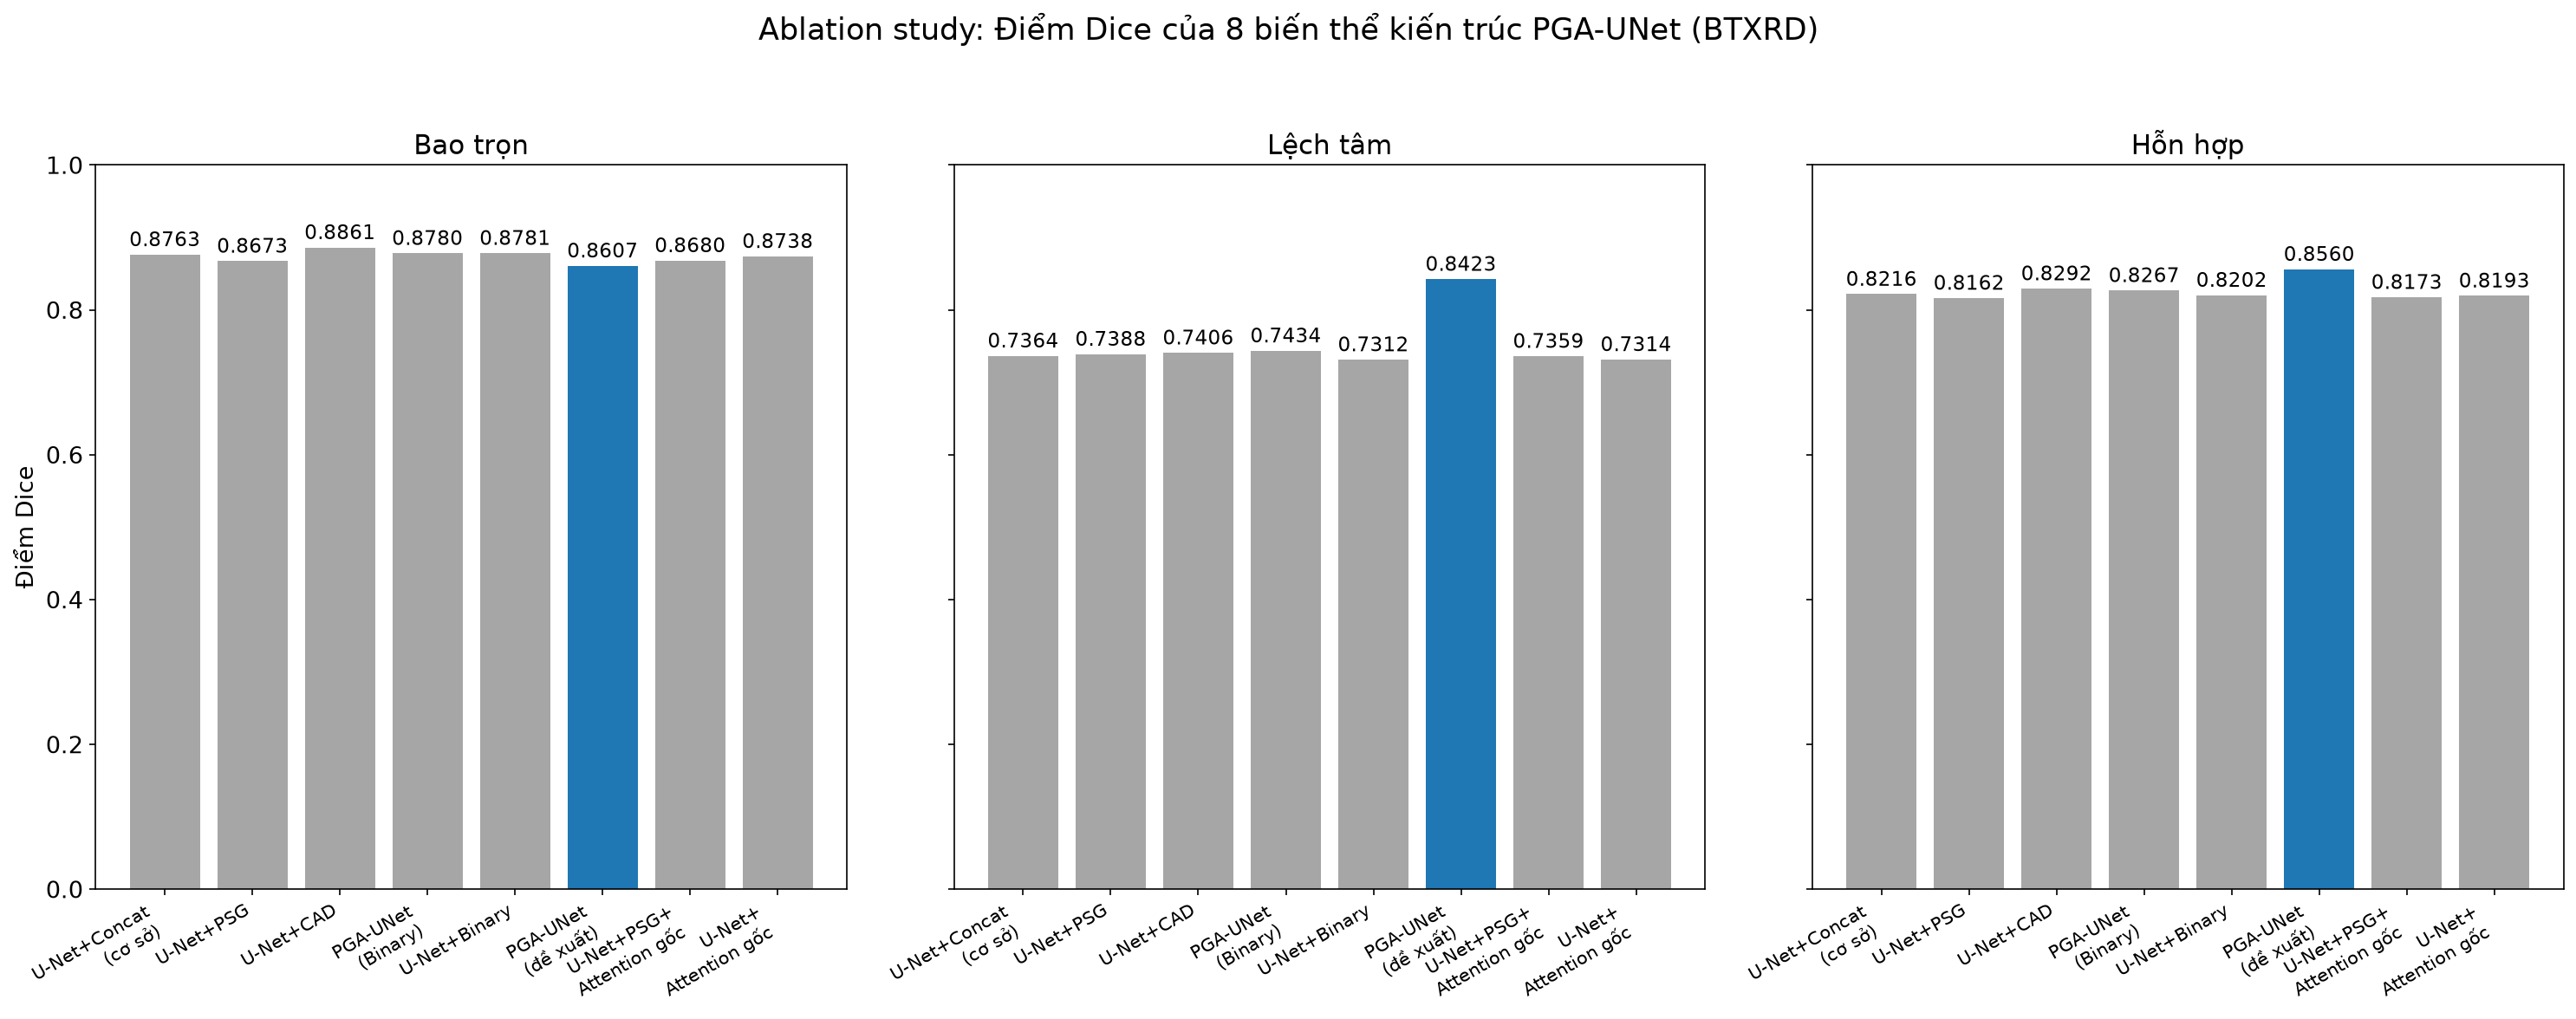
\includegraphics[width=0.95\textwidth]{images/chart_ablation.png}
    \caption{Dice của tám cấu hình trong nghiên cứu loại bỏ thành phần trên BTXRD. PGA-UNet đạt kết quả cao nhất trong hai kịch bản Lệch tâm và Hỗn hợp.}
    \label{fig:chart_ablation}
\end{figure}

Các nhận xét trên dựa vào sự chênh lệch Dice trung bình. Kiểm định Wilcoxon signed-rank trên Dice bắt cặp theo từng ảnh được trình bày tại Mục~\ref{subsec:conclusion_arch} để đánh giá độ tin cậy thống kê của các cặp so sánh chính.
% ------------------------------------------------------------
\subsection{Độ ổn định qua kiểm chứng chéo ngẫu nhiên lặp lại}
\label{subsec:cross_validation}
% ------------------------------------------------------------

PGA-UNet được đánh giá bằng kiểm chứng chéo ngẫu nhiên lặp lại 4 lần trên tập huấn luyện và xác thực. Ở mỗi lần, dữ liệu được xáo lại theo cấp độ ảnh, còn các đa giác thuộc cùng một ảnh luôn đi cùng nhau để tránh rò rỉ dữ liệu. Đây không phải là k-fold cross-validation theo nghĩa kỹ thuật chuẩn, mà là 4 lần chia ngẫu nhiên độc lập để xem kết quả có nhạy với cách chia dữ liệu hay không. Bảng~\ref{tab:cross_validation_per_fold} trình bày Dice trên từng lần, trong khi Bảng~\ref{tab:cross_validation} tổng hợp kết quả trung bình của sáu chỉ số đánh giá.

\begin{table}[H]
    \centering
    \caption{Dice của PGA-UNet trong kiểm chứng chéo ngẫu nhiên lặp lại 4 lần trên BTXRD (kịch bản Bao trọn / Lệch tâm / Hỗn hợp)}
    \label{tab:cross_validation_per_fold}
    \renewcommand{\arraystretch}{1.3}
    \resizebox{\textwidth}{!}{%
    \begin{tabular}{|c|c|c|c|}
        \hline
        \textbf{Lần} & \textbf{Bao trọn↑} & \textbf{Lệch tâm↑} & \textbf{Hỗn hợp↑} \\
        \hline
        1 & 0.8514 & 0.8206 & 0.8424 \\
        \hline
        2 & 0.8755 & 0.8534 & 0.8677 \\
        \hline
        3 & 0.8602 & 0.8414 & 0.8533 \\
        \hline
        4 & 0.8646 & 0.8426 & 0.8610 \\
        \hline
        \textbf{Trung bình ± độ lệch chuẩn} & $\mathbf{0.8629 \pm 0.0087}$ & $\mathbf{0.8395 \pm 0.0119}$ & $\mathbf{0.8561 \pm 0.0094}$ \\
        \hline
    \end{tabular}%
    }
\end{table}

Độ lệch chuẩn Dice dao động từ 0,0087 đến 0,0119, tức là khá nhỏ. Kịch bản Lệch tâm vẫn dao động nhiều nhất, điều này hợp lý vì chính cách tạo câu nhắc ở kịch bản này đã có yếu tố ngẫu nhiên. Bảng~\ref{tab:cross_validation} bổ sung các chỉ số còn lại (IoU, Precision, Recall, HD95, CBL) tính theo giá trị trung bình cho ba kịch bản trên.

\begin{table}[H]
    \centering
    \caption{Kết quả trung bình của kiểm chứng chéo ngẫu nhiên lặp lại 4 lần của PGA-UNet trên ba kịch bản câu nhắc}
    \label{tab:cross_validation}
    \renewcommand{\arraystretch}{1.3}
    \resizebox{\textwidth}{!}{%
    \begin{tabular}{|l|c|c|c|c|c|c|}
        \hline
        \textbf{Kịch bản} & \textbf{Dice↑} & \textbf{IoU↑} & \textbf{Precision↑} & \textbf{Recall↑} & \textbf{HD95↓} & \textbf{CBL↑} \\
        \hline
        Bao trọn & 0.8629 & 0.7672 & 0.8506 & 0.8910 & 11.14 & 0.9548 \\
        \hline
        Lệch tâm & 0.8395 & 0.7332 & 0.8393 & 0.8574 & 13.25 & 0.9381 \\
        \hline
        Hỗn hợp (70\% Bao trọn + 30\% Lệch tâm) & 0.8561 & 0.7573 & 0.8466 & 0.8820 & 11.90 & 0.9501 \\
        \hline
    \end{tabular}%
    }
\end{table}

Dice trung bình sau 4 lần ở Bao trọn là $0{,}8629$, rất gần với kết quả trên tập kiểm thử ở chương 4 (trong bảng~\ref{tab:baseline_comparison}) là $0{,}8607$. Điều đó cho thấy kết quả báo cáo không phải chỉ do may mắn từ một lần chia dữ liệu cụ thể.

Kiểm định Wilcoxon trên Dice bắt cặp theo từng ảnh được trình bày riêng tại Mục~\ref{subsec:conclusion_arch}; kiểm định này được thực hiện trực tiếp trên từng cặp ảnh tương ứng, hoàn toàn độc lập với biến động độ lệch chuẩn giữa các lần chạy.
% ------------------------------------------------------------
\subsection{Phân tích theo đặc tính tổn thương}
\label{subsec:subcategory}
% ------------------------------------------------------------

Mục này khảo sát sự thay đổi hiệu năng của PGA-UNet trên các nhóm ảnh có đặc điểm khác nhau. Ba phân tích được thực hiện gồm: so sánh với U-Net trên các ảnh mà U-Net hoạt động tốt hoặc kém trên độ phân giải $512\times512$. Ngoài ra còn so sánh với SAM-Med2D theo kích thước và mức độ rõ của tổn thương trên độ phân giải $256\times256$.

Các kết quả phân nhóm có vai trò bổ sung cho đánh giá trên toàn bộ tập kiểm thử. Do mỗi nhóm chỉ gồm một phần dữ liệu và được xác định theo tiêu chí riêng, kết quả không thay thế cho các chỉ số trung bình được báo cáo ở Mục~\ref{sec:danh_gia_hieu_nang} trong Chương~\ref{Chapter4}.

\noindent\textbf{So sánh với U-Net theo mức hiệu năng của mô hình cơ sở}\\
Từ tập kiểm thử BTXRD, 50 ảnh có Dice U-Net cao nhất được xếp vào nhóm U-Net hoạt động tốt, trong khi 50 ảnh có Dice thấp nhất được xếp vào nhóm U-Net hoạt động kém. Cách phân nhóm này nhằm khảo sát liệu PGA-UNet chỉ cải thiện trên những ảnh U-Net đã xử lý tốt hay vẫn duy trì kết quả trên các trường hợp U-Net gặp nhiều khó khăn.

Do nhóm được xác định trực tiếp từ kết quả của U-Net, đây là phân tích mô tả theo hai cực hiệu năng của mô hình cơ sở, không phải cách phân loại độ khó độc lập của dữ liệu.

\begin{table}[H]
    \centering
    \caption{So sánh PGA-UNet với U-Net theo mức hiệu năng của U-Net trên BTXRD (50 ảnh/nhóm)}
    \label{tab:subcat_baseline}
    \renewcommand{\arraystretch}{1.3}
    \resizebox{\textwidth}{!}{%
    \begin{tabular}{|l|l|c|c|c|c|c|c|}
        \hline
        \textbf{Nhóm}
        & \textbf{Mô hình}
        & \textbf{Dice↑}
        & \textbf{IoU↑}
        & \textbf{Precision↑}
        & \textbf{Recall↑}
        & \textbf{HD95↓ (px)}
        & \textbf{CBL↑} \\
        \hline
        \multirow{2}{*}{U-Net hoạt động tốt}
        & U-Net
        & 0.8488 & 0.7403 & 0.8481 & 0.8618 & 51.34 & 0.9194 \\
        & PGA-UNet
        & \textbf{0.8972}
        & \textbf{0.8160}
        & \textbf{0.8656}
        & \textbf{0.9368}
        & \textbf{13.20}
        & \textbf{0.9666} \\
        \hline
        \multirow{2}{*}{U-Net hoạt động kém}
        & U-Net
        & 0.0211 & 0.0111 & 0.0396 & 0.1063 & 284.72 & 0.0708 \\
        & PGA-UNet
        & \textbf{0.8261}
        & \textbf{0.7168}
        & \textbf{0.8313}
        & \textbf{0.8429}
        & \textbf{7.75}
        & \textbf{0.9456} \\
        \hline
    \end{tabular}%
    }
\end{table}

Trong nhóm U-Net hoạt động tốt, PGA-UNet cải thiện Dice từ 0,8488 lên 0,8972, tương ứng mức tăng 0,0484. Các chỉ số IoU, Precision, Recall và CBL cũng tăng, trong khi HD95 giảm từ 51,34 xuống 13,20 điểm ảnh. Có thể thấy câu nhắc vẫn có ích ngay cả trên những ảnh mà mô hình tự động đã phân đoạn tương đối tốt.

\vspace{0.3cm}

Ở nhóm U-Net hoạt động kém, Dice của U-Net chỉ đạt 0,0211, trong khi PGA-UNet đạt 0,8261. Recall tăng từ 0,1063 lên 0,8429 và HD95 giảm từ 284,72 xuống 7,75 điểm ảnh. Tức là PGA-UNet vẫn định vị và phân đoạn được tổn thương trên nhiều ảnh mà U-Net gần như bỏ sót.

Sự chênh lệch vượt trội ở nhóm thứ hai xuất phát từ chính tiêu chí lựa chọn: nhóm này gồm 50 ảnh mà U-Net cho kết quả Dice kém nhất. Do đó, thay vì dùng để ước tính mức cải thiện trung bình toàn cục, chỉ số này phản ánh khả năng khắc phục các trường hợp thất bại nghiêm trọng của PGA-UNet.

\begin{figure}[H]
    \centering
    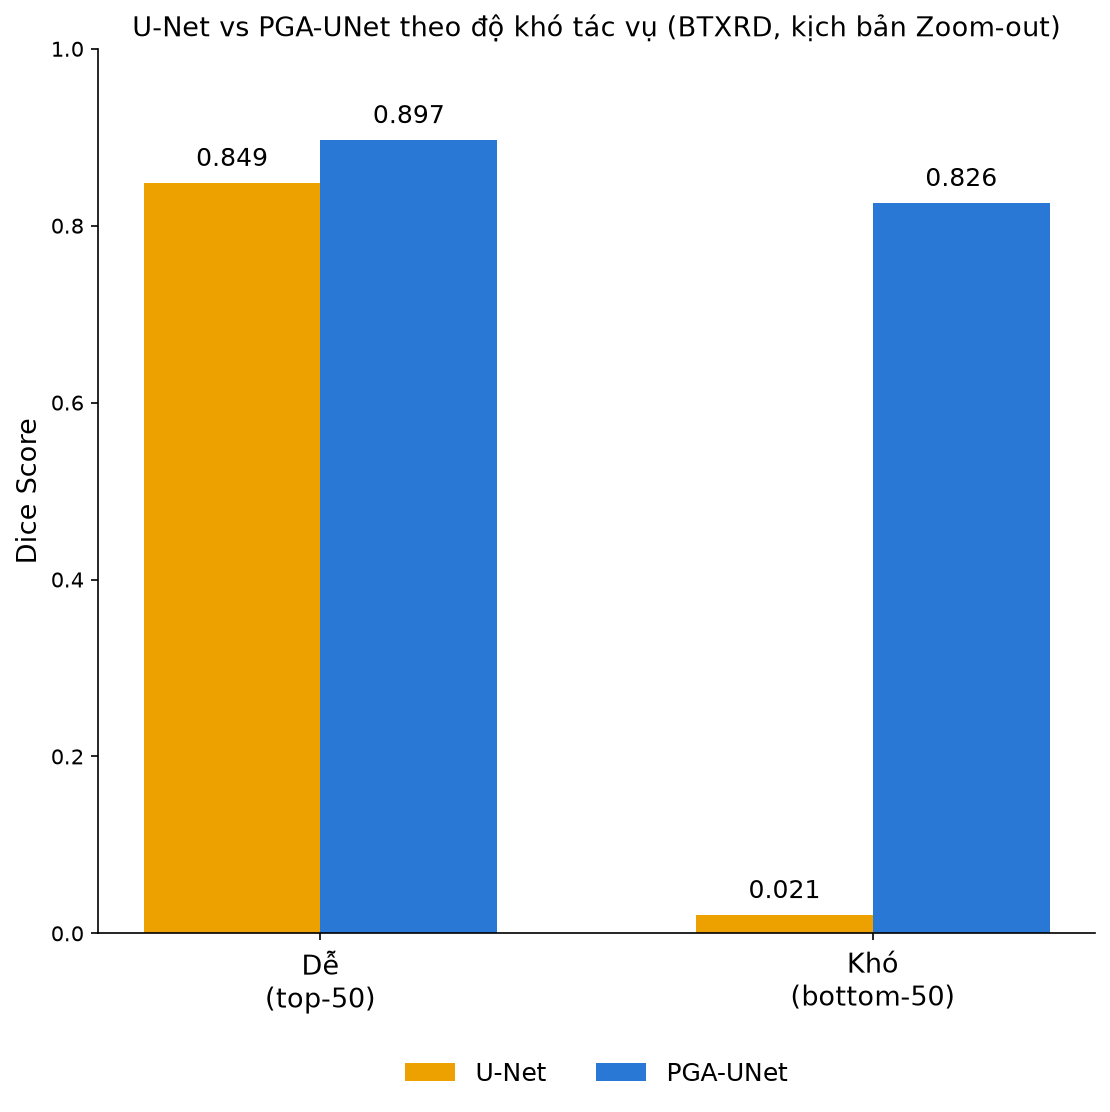
\includegraphics[width=0.5\textwidth]{images/chart_subcat_baseline_btxrd.png}
    \caption{Dice của U-Net và PGA-UNet trên nhóm U-Net hoạt động tốt và nhóm U-Net hoạt động kém.}
    \label{fig:chart_subcat_baseline_btxrd}
\end{figure}

Hình~\ref{fig:qual_subcat_baseline_btxrd} minh họa một ảnh thuộc mỗi nhóm. Như ở nhóm U-Net hoạt động tốt, Dice của U-Net và PGA-UNet lần lượt đạt 0,903 và 0,958. Còn ở nhóm U-Net hoạt động kém, U-Net không xác định được vùng tổn thương, trong khi PGA-UNet đạt Dice 0,901. Hai trường hợp này chỉ có vai trò minh họa cho xu hướng trong Bảng~\ref{tab:subcat_baseline}, không thay thế kết quả trên toàn bộ nhóm.

\begin{figure}[H]
    \centering
    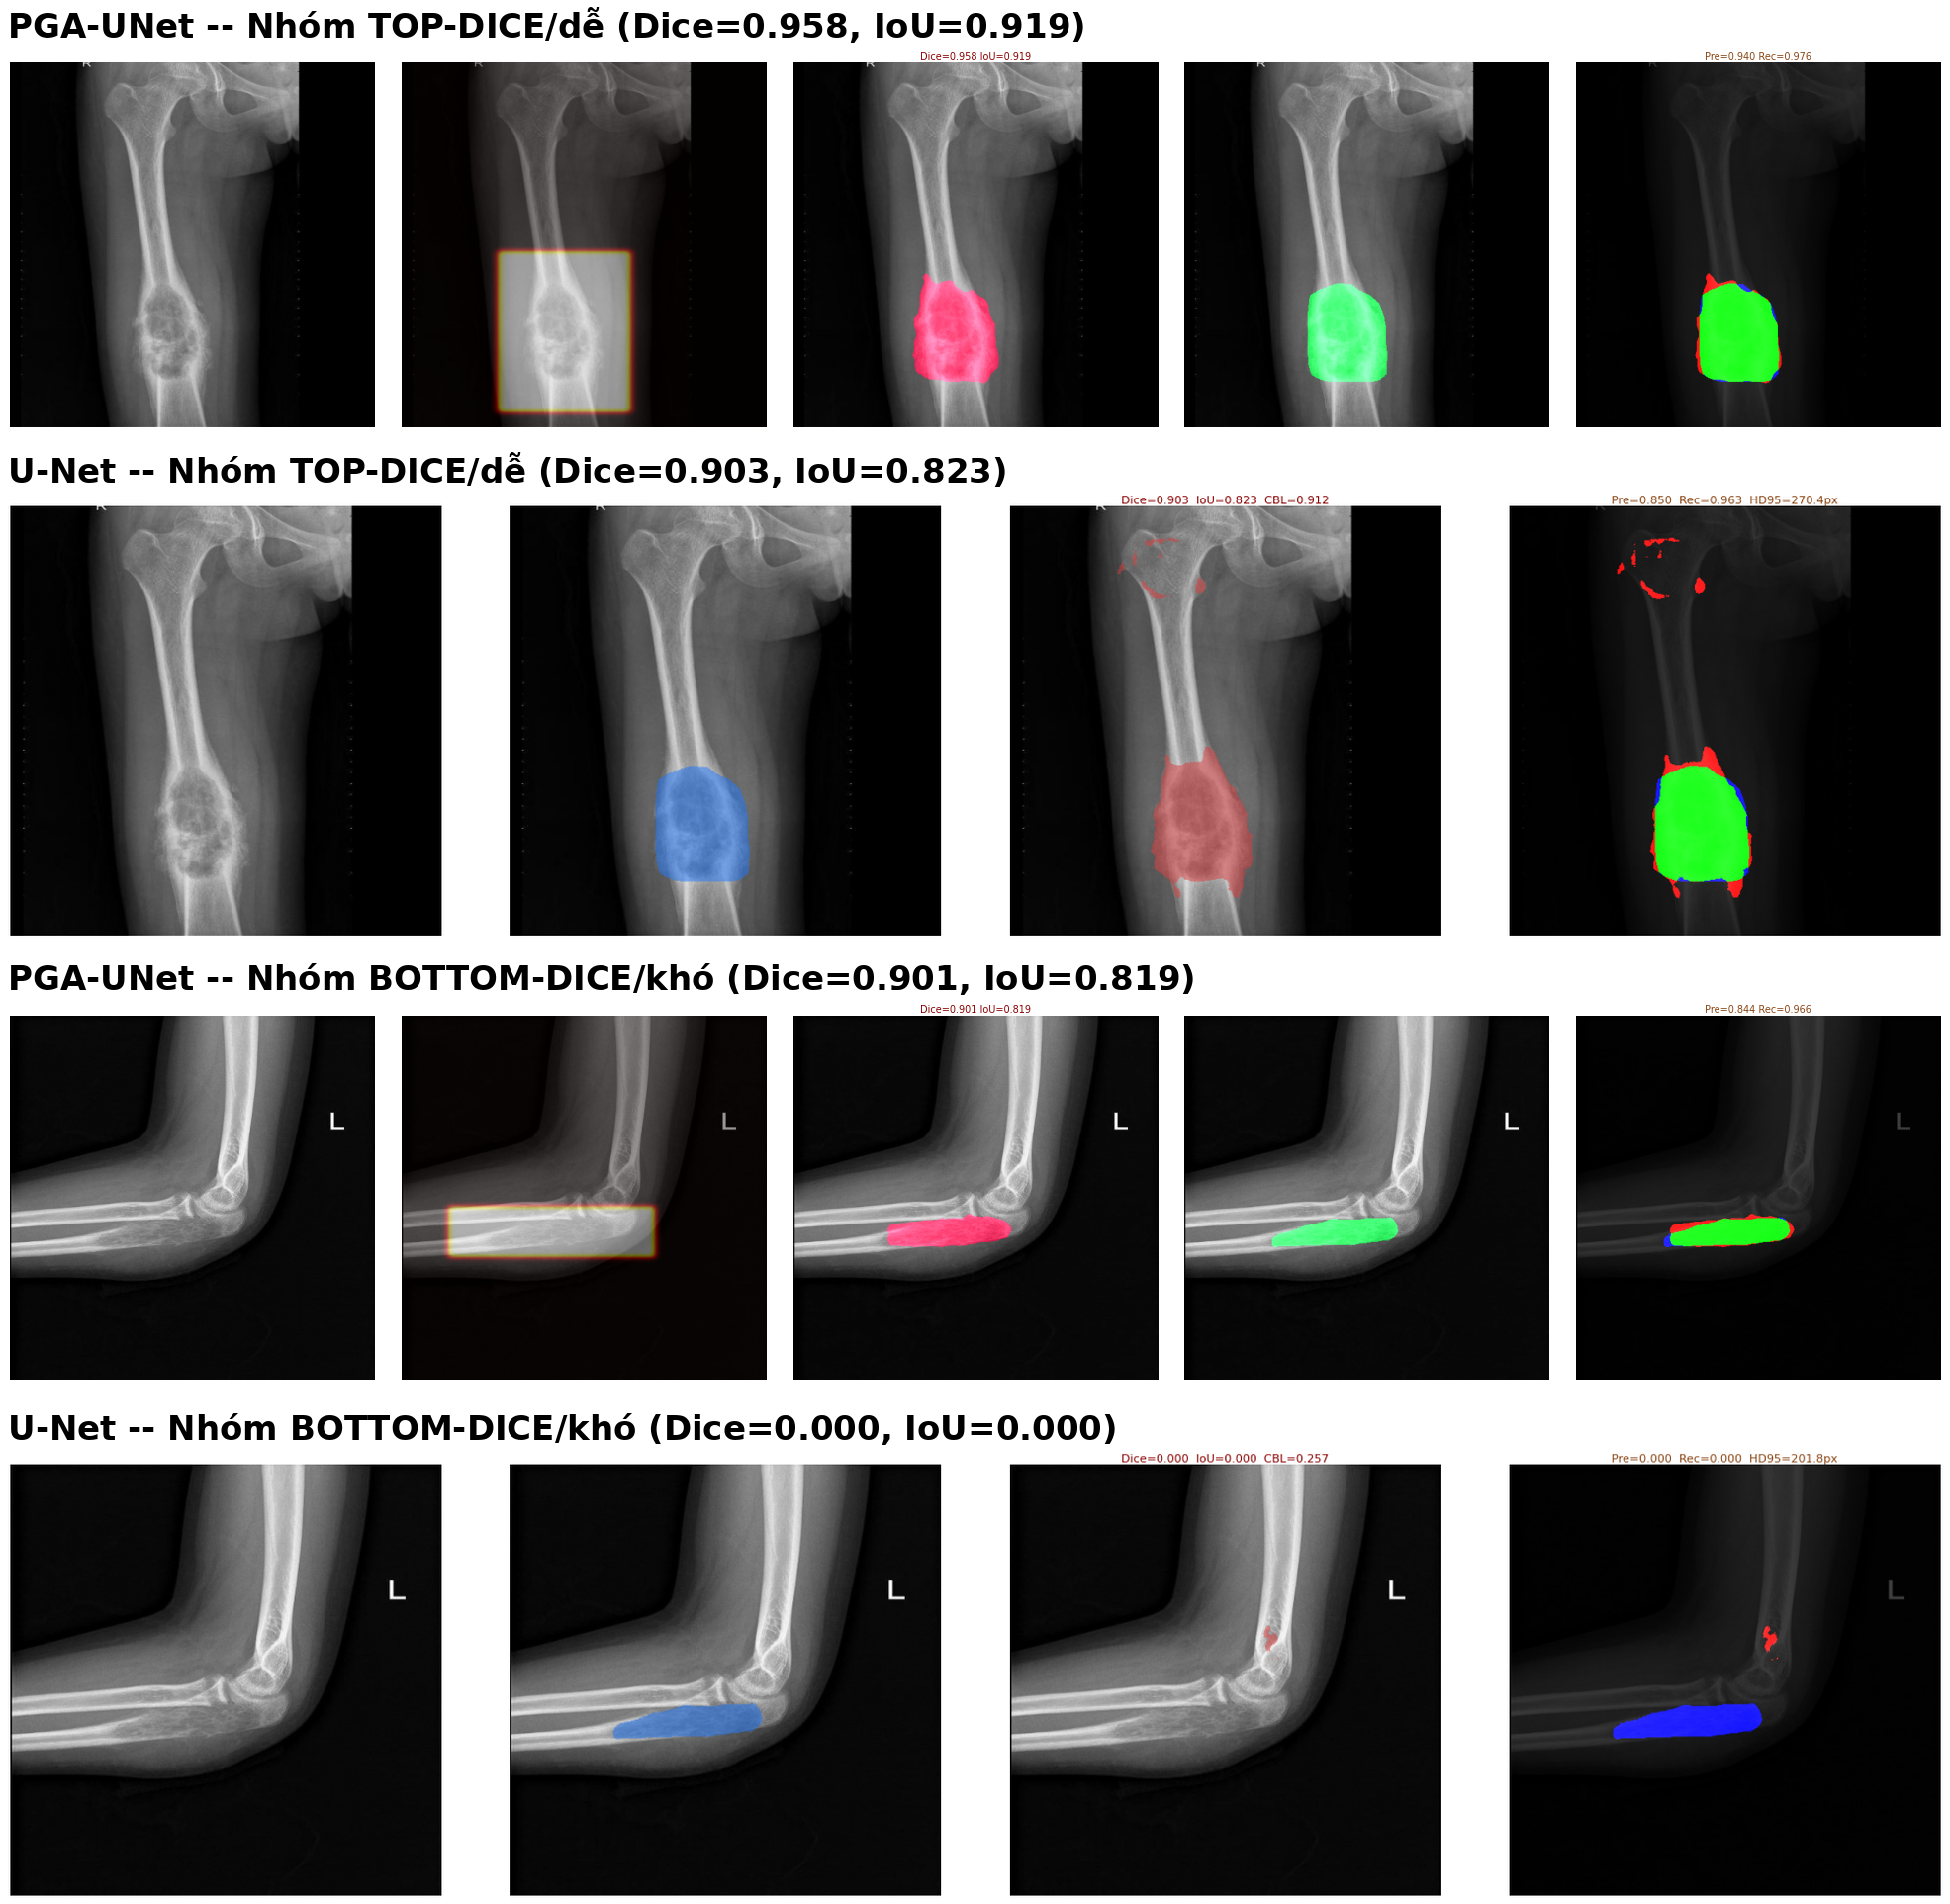
\includegraphics[width=0.8\textwidth]{images/qual_subcat_baseline_btxrd.png}
    \caption{Kết quả định tính của U-Net và PGA-UNet trên một ảnh thuộc mỗi nhóm hiệu năng của U-Net.}
    \label{fig:qual_subcat_baseline_btxrd}
\end{figure}

\noindent\textbf{So sánh với SAM-Med2D theo đặc tính tổn thương}\\
Để so sánh công bằng giữa hai kiến trúc, PGA-UNet và SAM-Med2D đều được đánh giá ở độ phân giải $256\times256$, trên cùng ba nhóm ảnh và cùng câu nhắc Bao trọn. Ba nhóm gồm Tổn thương nhỏ, Biên mờ và Tổn thương rõ, mỗi nhóm có 50 ảnh. Phép so sánh này chỉ thay đổi kiến trúc mô hình, không bị ảnh hưởng bởi sự khác biệt về độ phân giải đầu vào.

\begin{table}[H]
    \centering
    \caption{So sánh PGA-UNet với SAM-Med2D theo đặc tính tổn thương ở cùng độ phân giải $256\times256$ trên BTXRD (Bao trọn, 50 ảnh/nhóm)}
    \label{tab:subcat_sam_256}
    \renewcommand{\arraystretch}{1.3}
    \resizebox{\textwidth}{!}{%
    \begin{tabular}{|l|l|c|c|c|c|c|c|}
        \hline
        \textbf{Nhóm}
        & \textbf{Mô hình}
        & \textbf{Dice↑}
        & \textbf{IoU↑}
        & \textbf{Precision↑}
        & \textbf{Recall↑}
        & \textbf{HD95↓ (px)}
        & \textbf{CBL↑} \\
        \hline
        \multirow{2}{*}{Tổn thương nhỏ}
        & SAM-Med2D ($256\times256$)
        & 0.1356 & 0.0909 & 0.4331 & 0.0932 & 265.55 & 0.4257 \\
        & PGA-UNet ($256\times256$)
        & \textbf{0.6870}
        & \textbf{0.5383}
        & \textbf{0.5687}
        & \textbf{0.9354}
        & \textbf{5.98}
        & \textbf{0.9092} \\
        \hline
        \multirow{2}{*}{Biên mờ}
        & SAM-Med2D ($256\times256$)
        & 0.5759 & 0.4260 & \textbf{0.8866} & 0.4616 & 28.74 & 0.9000 \\
        & PGA-UNet ($256\times256$)
        & \textbf{0.7970}
        & \textbf{0.6715}
        & 0.7317
        & \textbf{0.8977}
        & \textbf{18.84}
        & \textbf{0.9397} \\
        \hline
        \multirow{2}{*}{Tổn thương rõ}
        & SAM-Med2D ($256\times256$)
        & 0.8529 & 0.7469 & \textbf{0.8807} & 0.8342 & 24.33 & 0.9587 \\
        & PGA-UNet ($256\times256$)
        & \textbf{0.8660}
        & \textbf{0.7669}
        & 0.8050
        & \textbf{0.9455}
        & \textbf{23.08}
        & \textbf{0.9599} \\
        \hline
    \end{tabular}%
    }
\end{table}

Mức chênh lệch giữa hai mô hình phụ thuộc rõ rệt vào đặc tính tổn thương. Ở nhóm Tổn thương nhỏ, PGA-UNet đạt Dice 0,6870, cao hơn 0,5514 so với SAM-Med2D. Recall của PGA-UNet đạt 0,9354, trong khi SAM-Med2D chỉ đạt 0,0932; đây cũng là nhóm tạo ra khoảng cách lớn nhất giữa hai mô hình.

Ở nhóm Biên mờ, PGA-UNet cao hơn SAM-Med2D 0,2211 Dice và 0,4361 Recall. SAM-Med2D đạt Precision cao hơn, nhưng Recall thấp cho thấy mô hình dự đoán thận trọng và bỏ sót nhiều điểm ảnh tổn thương hơn. Trong khi đó, PGA-UNet đạt sự cân bằng tốt hơn giữa khả năng bao phủ tổn thương và độ chính xác tổng thể.

Ở nhóm Tổn thương rõ, khoảng cách Dice thu hẹp còn 0,0131. Hai mô hình đều đạt kết quả cao khi vùng tổn thương dễ nhận biết; PGA-UNet cao hơn về Dice, IoU và Recall, trong khi SAM-Med2D cao hơn về Precision. Nhìn chung, ưu thế của PGA-UNet thể hiện rõ nhất trên tổn thương nhỏ và biên mờ, còn ở tổn thương rõ ràng thì hai mô hình gần nhau hơn.

\begin{figure}[H]
    \centering
    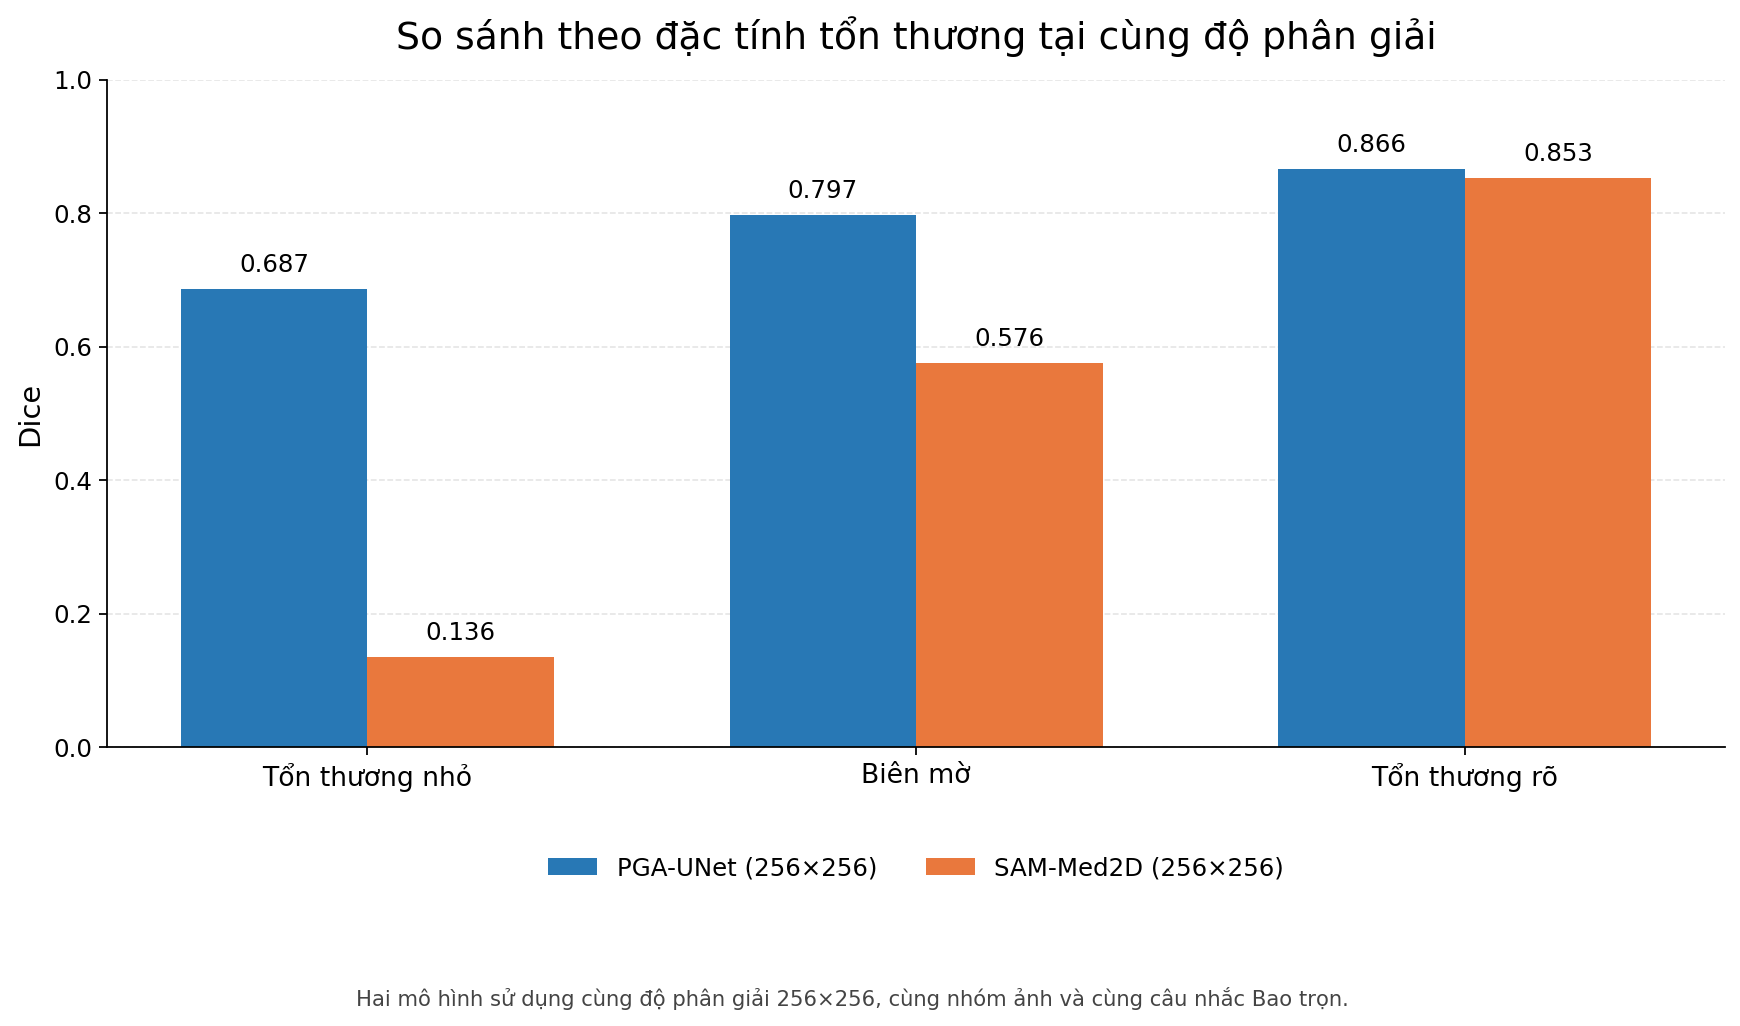
\includegraphics[width=0.9\textwidth]{images/chart_subcat_pga256_sam256_btxrd.png}
    \caption{So sánh Dice của PGA-UNet và SAM-Med2D theo đặc tính tổn thương ở cùng độ phân giải $256\times256$ trên BTXRD.}
    \label{fig:chart_subcat_pga256_sam256_btxrd}
\end{figure}

Hình~\ref{fig:qual_subcat_sam_btxrd} minh họa một ảnh đại diện cho mỗi nhóm, đối chiếu cả ba cấu hình SAM-Med2D, PGA-UNet$_{256}$ và PGA-UNet$_{512}$. Các ảnh được chọn theo tiêu chí Dice và IoU tăng dần đơn điệu qua ba cấu hình (SAM-Med2D~$<$~PGA-UNet$_{256}$~$<$~PGA-UNet$_{512}$), nhằm minh họa trực quan đồng thời cả lợi thế kiến trúc so với SAM-Med2D lẫn lợi ích của độ phân giải cao hơn được phân tích tại Mục~\ref{subsec:summary_subcat} của Chương~\ref{Chapter4} và ngay bên dưới.

\begin{figure}[H]
    \centering
    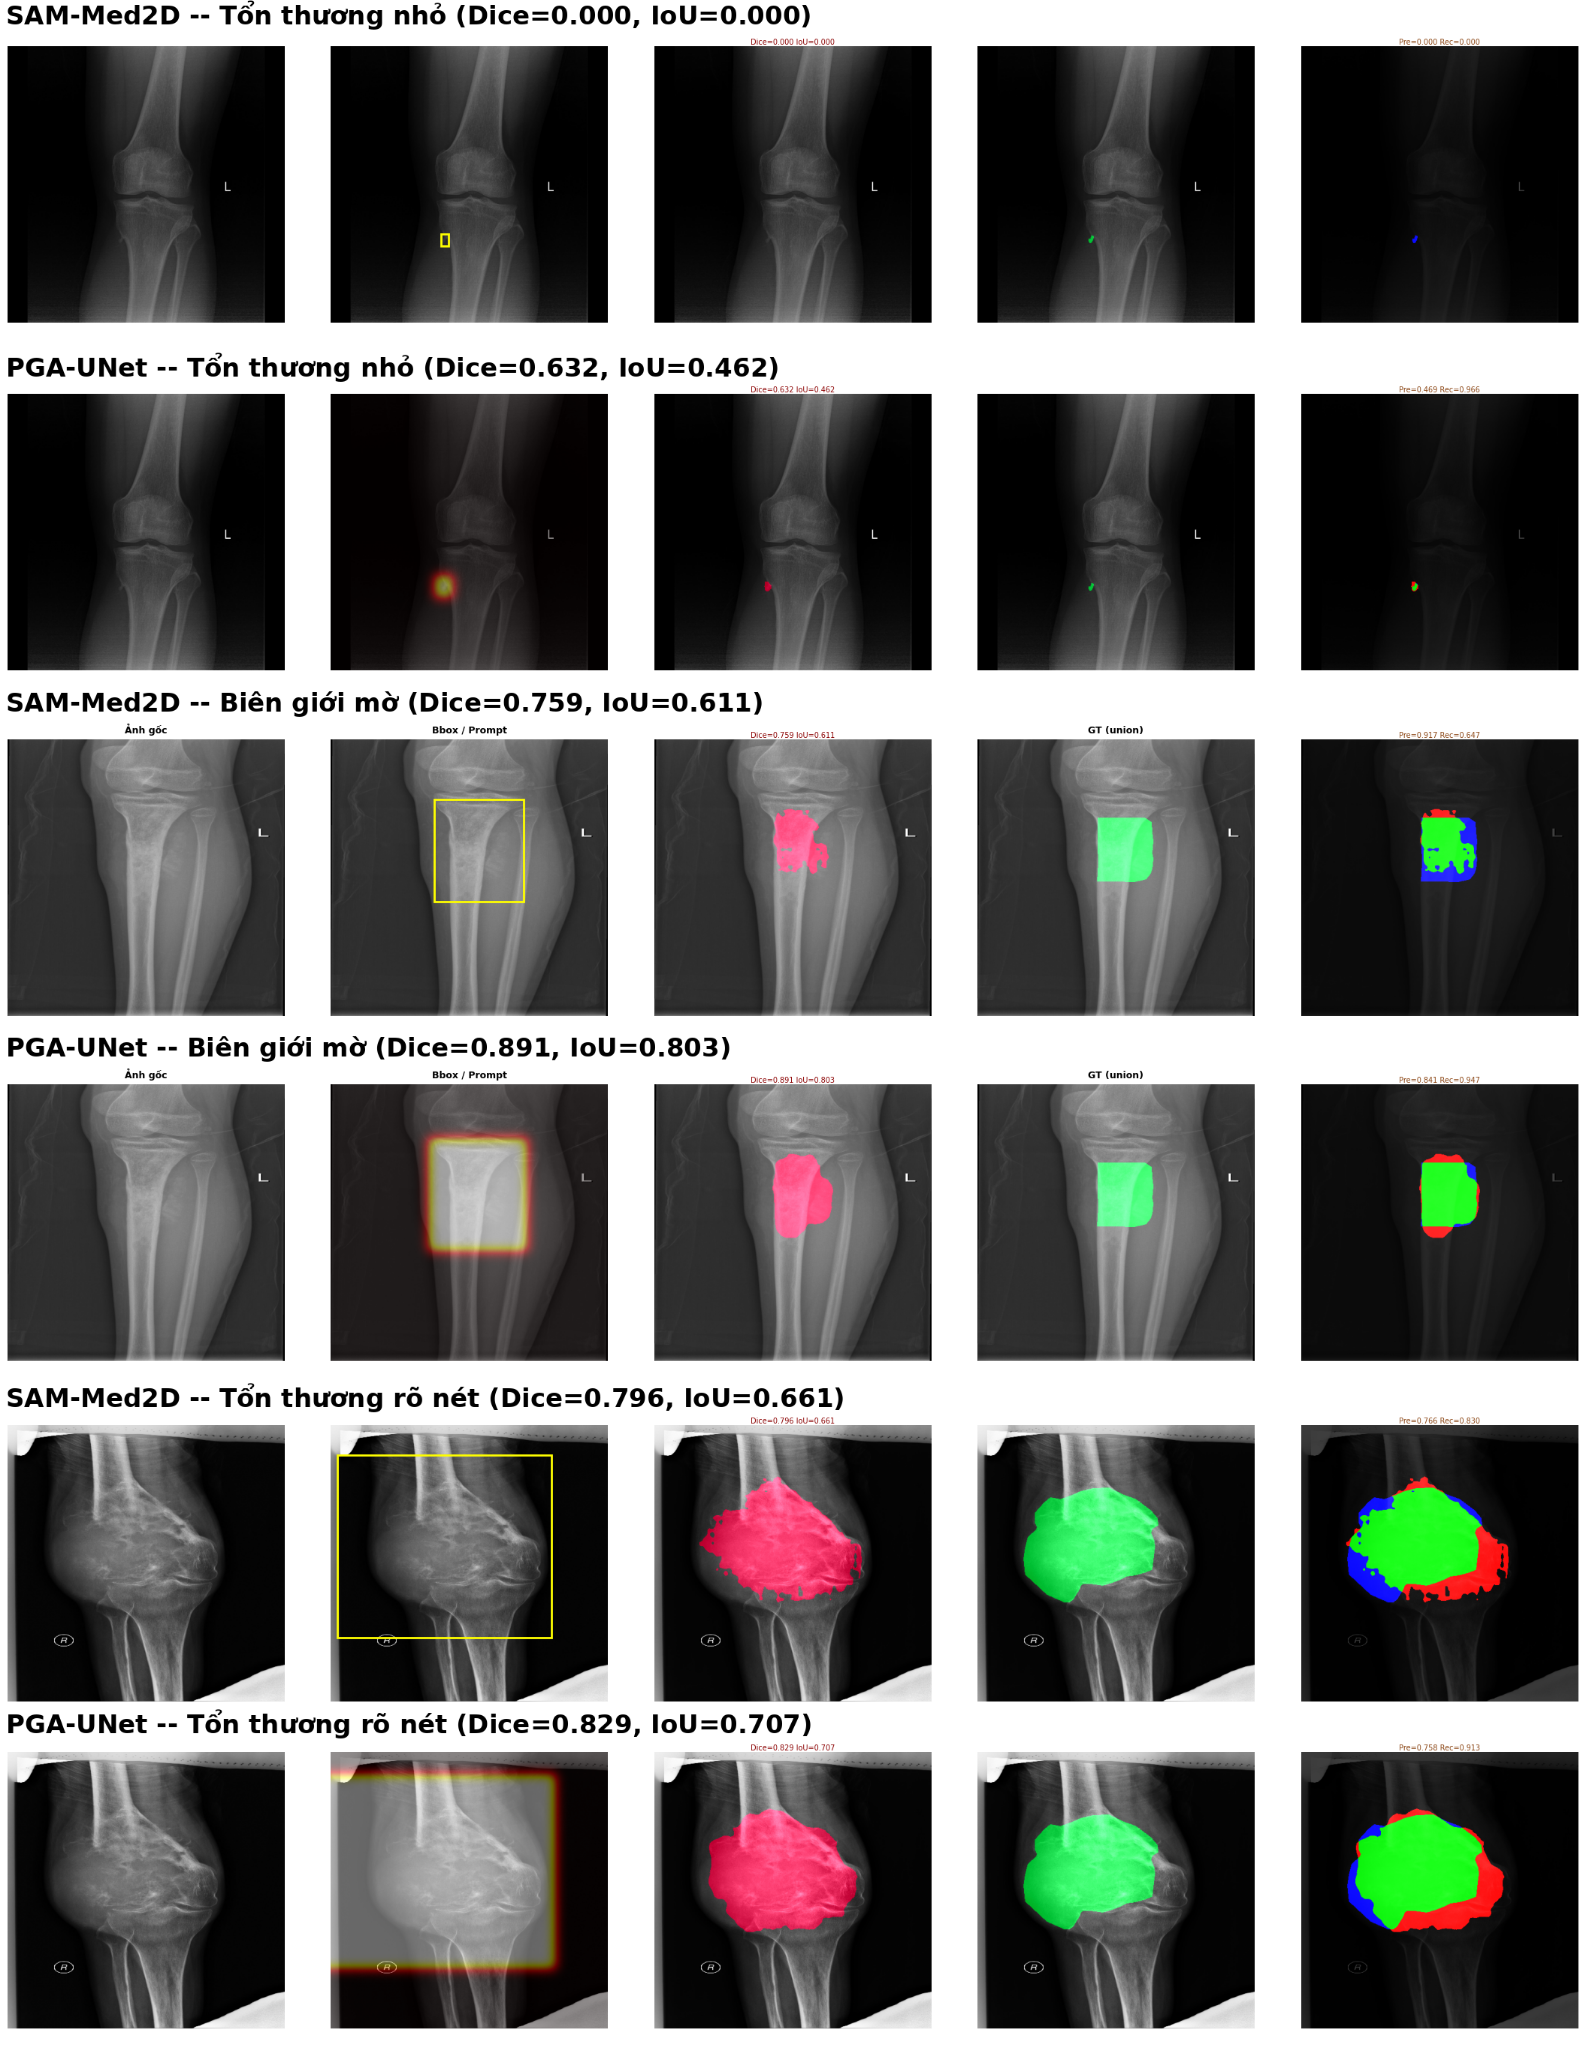
\includegraphics[width=\textwidth,height=0.87\textheight,keepaspectratio]{images/qual_subcat_sam_btxrd.png}
    \caption{Kết quả định tính của SAM-Med2D, PGA-UNet$_{256}$ và PGA-UNet$_{512}$ trên một ảnh đại diện mỗi nhóm đặc tính tổn thương, BTXRD.}
    \label{fig:qual_subcat_sam_btxrd}
\end{figure}

\noindent\textbf{Ảnh hưởng của độ phân giải theo đặc tính tổn thương}\\
Sau khi kiểm soát độ phân giải trong phép so sánh với SAM-Med2D, hai phiên bản PGA-UNet được đối chiếu trên cùng ba nhóm ảnh để xác định nhóm tổn thương nào cải thiện nhiều nhất khi tăng kích thước đầu vào từ $256\times256$ lên $512\times512$. Hai cấu hình sử dụng cùng kiến trúc, cùng nhóm mẫu và cùng câu nhắc Bao trọn; yếu tố thay đổi duy nhất là độ phân giải đầu vào và điểm lưu trọng số tương ứng.

\begin{table}[H]
    \centering
    \caption{Ảnh hưởng của độ phân giải đối với PGA-UNet theo đặc tính tổn thương trên BTXRD (Bao trọn, 50 ảnh/nhóm)}
    \label{tab:subcat_pga_resolution}
    \renewcommand{\arraystretch}{1.3}
    \resizebox{\textwidth}{!}{%
    \begin{tabular}{|l|l|c|c|c|c|c|c|}
        \hline
        \textbf{Nhóm}
        & \textbf{Độ phân giải}
        & \textbf{Dice↑}
        & \textbf{IoU↑}
        & \textbf{Precision↑}
        & \textbf{Recall↑}
        & \textbf{HD95 (px)}
        & \textbf{CBL↑} \\
        \hline
        \multirow{2}{*}{Tổn thương nhỏ}
        & $256\times256$
        & 0.6870 & 0.5383 & 0.5687 & \textbf{0.9354} & 5.98 & 0.9092 \\
        & $512\times512$
        & \textbf{0.8301}
        & \textbf{0.7212}
        & \textbf{0.8285}
        & 0.8553
        & 3.06
        & \textbf{0.9408} \\
        \hline
        \multirow{2}{*}{Biên mờ}
        & $256\times256$
        & 0.7970 & 0.6715 & 0.7317 & \textbf{0.8977} & 18.84 & 0.9397 \\
        & $512\times512$
        & \textbf{0.8448}
        & \textbf{0.7421}
        & \textbf{0.8527}
        & 0.8552
        & 13.87
        & \textbf{0.9546} \\
        \hline
        \multirow{2}{*}{Tổn thương rõ}
        & $256\times256$
        & 0.8660 & 0.7669 & 0.8050 & \textbf{0.9455} & 23.08 & 0.9599 \\
        & $512\times512$
        & \textbf{0.8826}
        & \textbf{0.7925}
        & \textbf{0.8477}
        & 0.9261
        & 22.79
        & \textbf{0.9629} \\
        \hline
    \end{tabular}%
    }
\end{table}

\textit{Lưu ý:} HD95 được tính theo đơn vị điểm ảnh tại từng độ phân giải nên không được dùng để so sánh trực tiếp giữa ảnh $256\times256$ và $512\times512$. Vì vậy, các giá trị HD95 trong Bảng~\ref{tab:subcat_pga_resolution} không được in đậm.

Việc tăng độ phân giải giúp PGA-UNet cải thiện Dice trên cả ba nhóm, nhưng mức cải thiện không đồng đều. Nhóm Tổn thương nhỏ cải thiện nhiều nhất, với Dice tăng từ 0,6870 lên 0,8301, tương ứng 0,1431. Precision đồng thời tăng từ 0,5687 lên 0,8285, cho thấy độ phân giải cao giúp mô hình hạn chế các vùng dự đoán nhầm quanh tổn thương nhỏ.

Ở nhóm Biên mờ, Dice tăng 0,0478 và Precision tăng 0,1210. Đối với nhóm Tổn thương rõ, Dice chỉ tăng 0,0166 vì cả hai độ phân giải đều đã đạt hiệu năng cao. Xu hướng này cho thấy độ phân giải cao đặc biệt hữu ích đối với các tổn thương nhỏ và khó phân biệt, trong khi chênh lệch giảm dần khi vùng tổn thương đã rõ ràng.

Recall của phiên bản $256\times256$ cao hơn trong cả ba nhóm, trong khi phiên bản $512\times512$ đạt Precision, Dice và CBL cao hơn. Kết quả cho thấy rằng phiên bản độ phân giải thấp có xu hướng bao phủ rộng hơn, còn phiên bản độ phân giải cao tạo mặt nạ chọn lọc và cân bằng hơn. Đây là xu hướng quan sát từ các chỉ số, không phải kết luận trực tiếp về cơ chế bên trong của mô hình.

\begin{figure}[H]
    \centering
    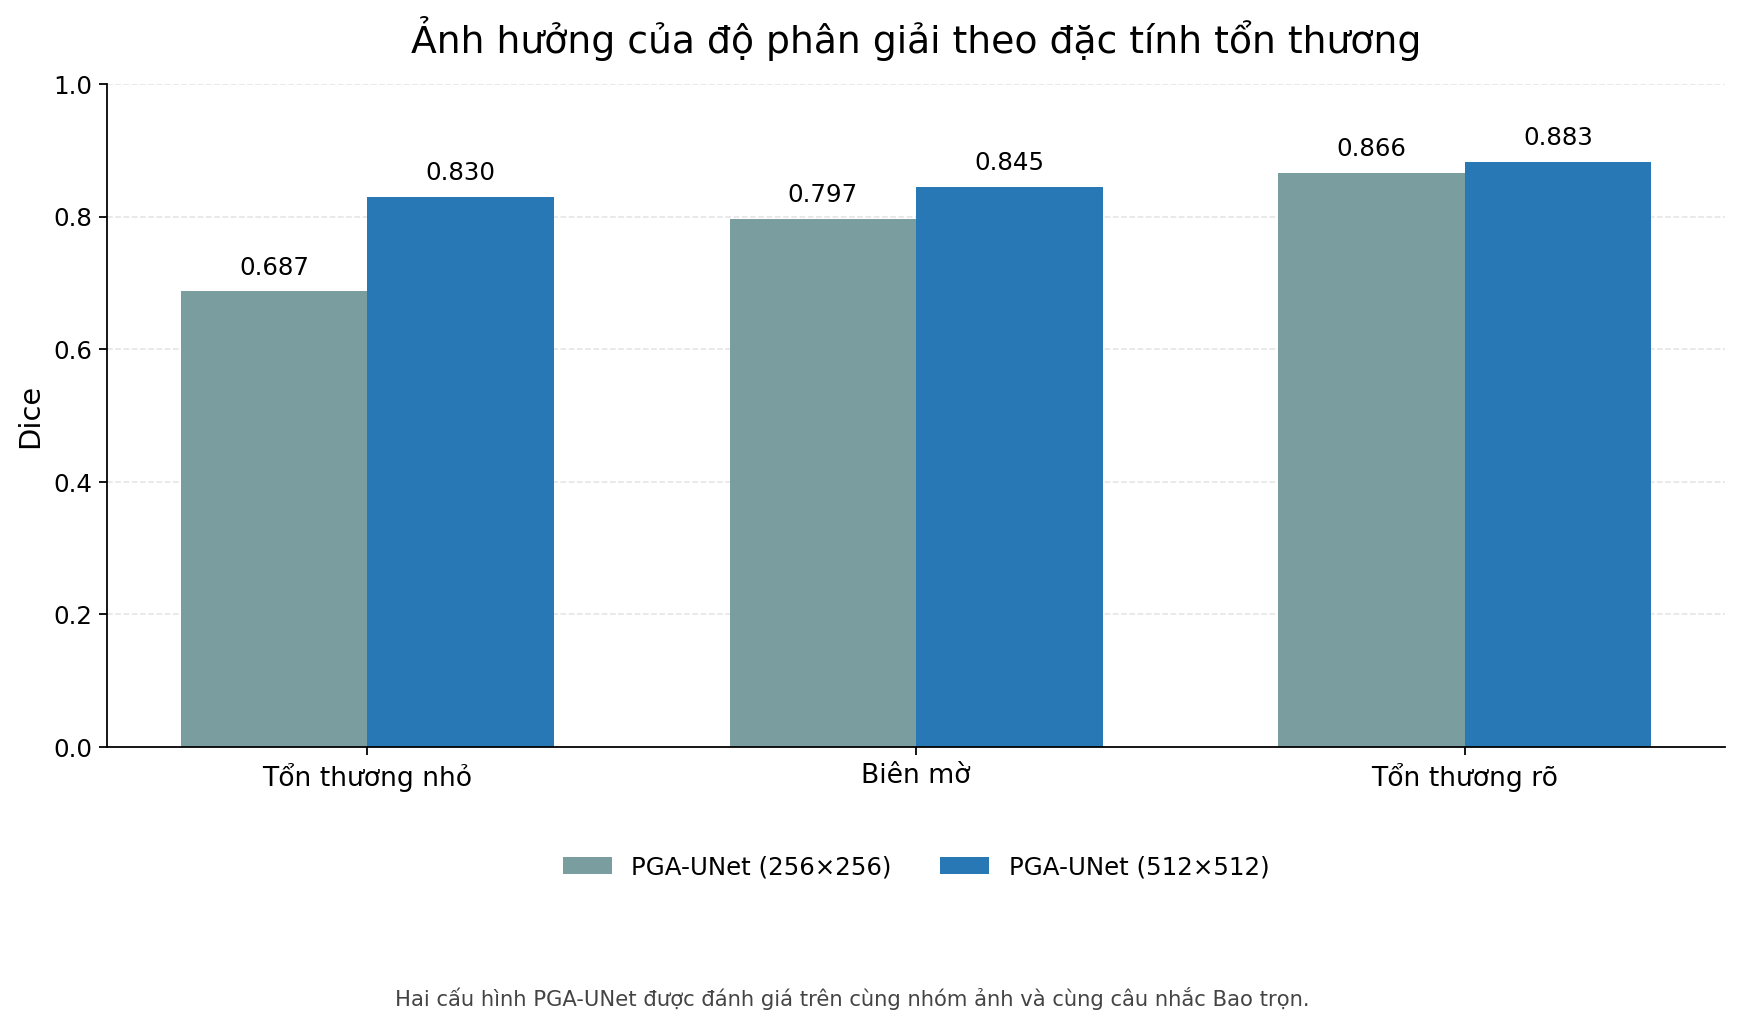
\includegraphics[width=0.8\textwidth]{images/chart_subcat_pga_resolution_btxrd.png}
    \caption{Ảnh hưởng của độ phân giải đến Dice của PGA-UNet theo ba nhóm đặc tính tổn thương trên BTXRD.}
    \label{fig:chart_subcat_pga_resolution_btxrd}
\end{figure}

\begin{figure}[H]
    \centering
    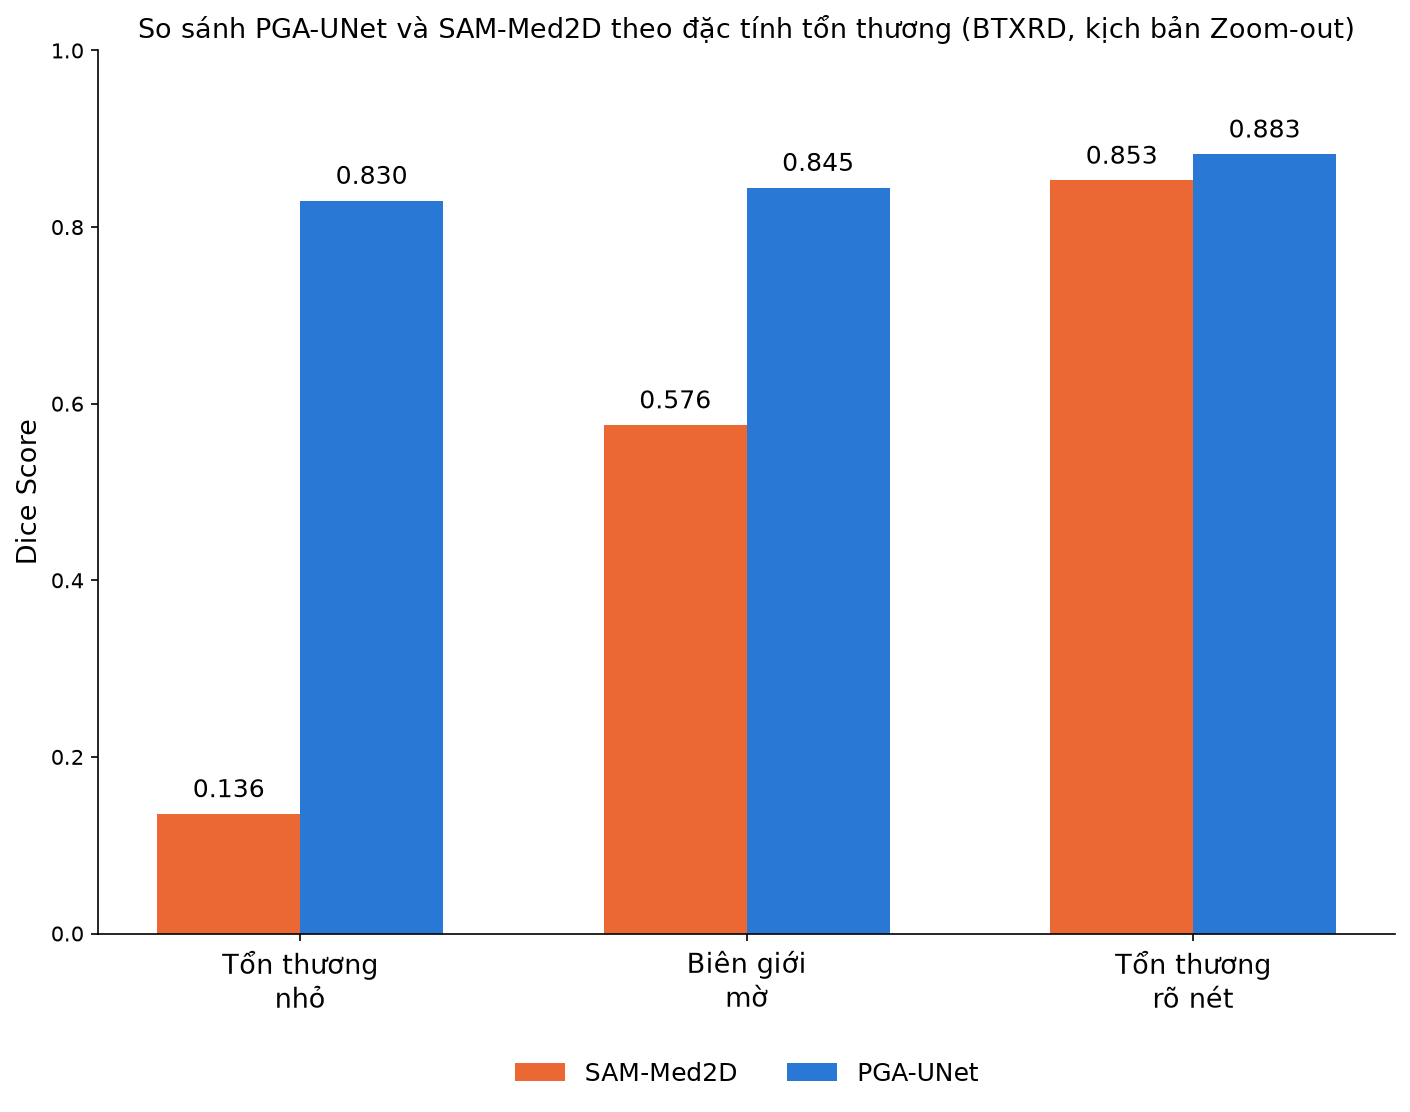
\includegraphics[width=0.9\textwidth]{images/chart_subcat_btxrd.png}
    \caption{Tổng hợp Dice của SAM-Med2D và PGA-UNet (256$\times$256, 512$\times$512) theo ba nhóm đặc tính tổn thương trên BTXRD.}
    \label{fig:chart_subcat_btxrd}
\end{figure}

\noindent\textbf{Kết luận}\\
Khi kiểm soát độ phân giải ở $256\times256$, PGA-UNet vẫn cao hơn SAM-Med2D trên cả ba nhóm, đặc biệt ở Tổn thương nhỏ và Biên mờ. Còn khi chỉ thay đổi độ phân giải của PGA-UNet, mức cải thiện lớn nhất vẫn rơi vào nhóm Tổn thương nhỏ. Kết hợp hai kết quả này cho thấy lợi thế của PGA-UNet trên nhóm này không chỉ đến từ độ phân giải $512\times512$, dù độ phân giải cao vẫn mang lại thêm cải thiện.
% ------------------------------------------------------------
\section{Phân tích trên FracAtlas}
\label{subsec:arch_fracatlas}
% ------------------------------------------------------------

Ba nhóm thí nghiệm trên được lặp lại với tập FracAtlas. Đây là bộ dữ liệu gãy xương nên hình thái tổn thương khác khá nhiều so với khối u xương của BTXRD. Tất cả mô hình đều được huấn luyện lại từ đầu, không dùng lại trọng số từ BTXRD. Mục tiêu ở đây không phải kiểm tra tổng quát hóa liên miền theo kiểu huấn luyện ở một tập dữ liệu rồi suy luận trên dữ liệu chưa từng thấy, mà là xem thiết kế của PGA-UNet có lặp lại được xu hướng hay chỉ là trùng hợp ngẫu nhiên trên tập BTXRD.

\subsection{Đóng góp của kiến trúc và câu nhắc}
\label{subsec:fracatlas_ablation}

\noindent\textbf{Thiết kế thí nghiệm}\\
Tám cấu hình trong Mục~\ref{subsec:ablation_arch} được huấn luyện lại từ đầu trên FracAtlas với cùng cách phân chia dữ liệu và cấu hình huấn luyện. Các cấu hình chỉ khác nhau ở sự hiện diện của PSG, cơ chế chú ý trên các kết nối tắt của nhánh giải mã và biểu diễn câu nhắc. Kết quả trong ba kịch bản được trình bày tại Bảng~\ref{tab:fracatlas_ablation_arch}.

\begin{table}[H]
    \centering
    \caption{Kết quả chỉ số Dice của nghiên cứu loại bỏ thành phần trên FracAtlas trong ba kịch bản câu nhắc (N=\NtestimgFA~ảnh)}
    \label{tab:fracatlas_ablation_arch}
    \renewcommand{\arraystretch}{1.3}
    \resizebox{\textwidth}{!}{%
    \begin{tabular}{|l|c|c|c|c|c|c|}
        \hline
        \textbf{Cấu hình}
        & \textbf{PSG}
        & \textbf{Chú ý trên kết nối tắt}
        & \textbf{Câu nhắc}
        & \textbf{Bao trọn↑}
        & \textbf{Lệch tâm↑}
        & \textbf{Hỗn hợp↑} \\
        \hline
        U-Net+Concat (Gaussian)
        & \texttimes & Không & Gaussian
        & 0.8131 & 0.6579 & 0.7573 \\
        \hline
        U-Net+PSG
        & \checkmark & Không & Gaussian
        & 0.8211 & 0.6760 & 0.7700 \\
        \hline
        U-Net+CAD
        & \texttimes & CAD & Gaussian
        & 0.7806 & 0.6551 & 0.7271 \\
        \hline
        PGA-UNet (nhị phân)
        & \checkmark & CAD & Nhị phân
        & 0.7907 & 0.6845 & 0.7474 \\
        \hline
        U-Net+Concat (nhị phân)
        & \texttimes & Không & Nhị phân
        & 0.8203 & 0.6630 & 0.7658 \\
        \hline
        \textbf{PGA-UNet}
        & \checkmark & CAD & Gaussian
        & 0.8169 & \textbf{0.7850} & \textbf{0.8129} \\
        \hline
        U-Net+PSG+Cổng chú ý nguyên bản
        & \checkmark & Nguyên bản & Gaussian
        & \textbf{0.8351} & 0.6927 & 0.7838 \\
        \hline
        U-Net+Cổng chú ý nguyên bản
        & \texttimes & Nguyên bản & Gaussian
        & 0.7896 & 0.6630 & 0.7378 \\
        \hline
    \end{tabular}%
    }
\end{table}

\noindent\textbf{Đối chiếu với các mô hình không sử dụng câu nhắc}\\
Trên FracAtlas, U-Net và Attention U-Net không sử dụng câu nhắc lần lượt đạt Dice 0,3831 và 0,2467 (Ở bảng~\ref{tab:fracatlas_baseline}). Trong khi đó, cấu hình nối kênh đơn giản U-Net+Concat đạt 0,8131 ở kịch bản Bao trọn. Điều này cho thấy thông tin vị trí từ câu nhắc đóng vai trò khá quan trọng khi phân đoạn đường gãy xương.

Tương tự với tập BTXRD, chỉ số Dice của Attention U-Net cũng thấp hơn U-Net trên tập FracAtlas. Kết quả cho thấy cổng chú ý nguyên bản không tự cải thiện hiệu năng trong thiết lập thiếu câu nhắc, điều này không trực tiếp xác định nguyên nhân gây suy giảm.

\noindent\textbf{Đóng góp của PSG tại bộ mã hóa}\\
So với U-Net+Concat, U-Net+PSG cải thiện Dice trong cả ba kịch bản: tăng 0,0080 ở Bao trọn, 0,0181 ở Lệch tâm và 0,0127 ở Hỗn hợp. Mức cải thiện này lớn hơn xu hướng đã quan sát được trên BTXRD, đồng thời cho thấy việc đưa thông tin không gian vào bộ mã hóa có lợi đối với các vùng gãy xương nhỏ và mảnh.

Tuy nhiên, U-Net+PSG vẫn thấp hơn PGA-UNet 0,1090 ở Lệch tâm và 0,0429 ở Hỗn hợp. Điều này cho thấy PSG giúp cải thiện đặc trưng mã hóa. Nhưng hiệu quả sẽ bị giới hạn nếu các kết nối tắt của nhánh giải mã không tiếp tục dùng thông tin câu nhắc này.

\noindent\textbf{Đóng góp của CAD và sự khác biệt với cổng chú ý nguyên bản}\\
Khi hoạt động không có PSG, U-Net+CAD không cải thiện so với U-Net+Concat. Dice giảm 0,0325 ở Bao trọn, 0,0028 ở Lệch tâm và 0,0302 ở Hỗn hợp. Có thể thấy CAD một mình chưa phát huy hiệu quả khi đặc trưng mã hóa chưa được PSG điều biến theo câu nhắc.

Cổng chú ý nguyên bản cũng phụ thuộc vào PSG. Khi không có PSG, U-Net+Cổng chú ý nguyên bản thấp hơn U-Net+Concat 0,0235 ở Bao trọn và 0,0195 ở Hỗn hợp, còn Lệch tâm chỉ tăng 0,0051. Khi bổ sung PSG, U-Net+PSG+Cổng chú ý nguyên bản đạt 0,8351 ở Bao trọn, 0,6927 ở Lệch tâm và 0,7838 ở Hỗn hợp, cao hơn cấu hình chỉ có PSG trong cả ba trường hợp.

So với cổng chú ý nguyên bản có PSG, PGA-UNet sử dụng CAD thấp hơn 0,0182 ở Bao trọn nhưng cao hơn 0,0923 ở Lệch tâm và 0,0291 ở Hỗn hợp. Cổng chú ý nguyên bản phù hợp hơn khi hộp giới hạn lý tưởng, còn CAD có ích rõ hơn khi câu nhắc bị lệch.

\noindent\textbf{Đóng góp của bản đồ nhiệt Gaussian}\\
Ở cấu hình nối kênh cơ sở, mặt nạ nhị phân cao hơn bản đồ Gaussian 0,0072 ở Bao trọn, 0,0051 ở Lệch tâm và 0,0085 ở Hỗn hợp. Các mức chênh lệch đều nhỏ hơn 0,01, cho thấy cách biểu diễn câu nhắc ít ảnh hưởng khi câu nhắc chỉ được nối trực tiếp vào đầu vào.

Khi kết hợp đầy đủ PSG và CAD, xu hướng thay đổi rõ rệt. PGA-UNet sử dụng Gaussian cao hơn phiên bản dùng câu nhắc nhị phân 0,0262 ở Bao trọn, 0,1005 ở Lệch tâm và 0,0655 ở Hỗn hợp. Qua đó có thể thấy lợi ích của Gaussian chỉ thực sự rõ khi thông tin câu nhắc được đưa vào cả bộ mã hóa qua PSG lẫn các kết nối tắt của nhánh giải mã qua CAD.

\noindent\textbf{Sự bổ trợ giữa PSG, CAD và bản đồ nhiệt Gaussian}\\
Trong kịch bản Lệch tâm, PSG riêng lẻ cải thiện 0,0181 so với U-Net+Concat, trong khi CAD riêng lẻ giảm 0,0028. Ngược lại, cấu hình đầy đủ PSG+CAD+Gaussian cải thiện 0,1271, từ 0,6579 lên 0,7850. Điều này cho thấy CAD không hoạt động hiệu quả như một thành phần độc lập, mà cần đặc trưng đã được PSG điều biến tại bộ mã hóa từ trước.

Theo thiết kế của PGA-UNet, PSG đưa thông tin vị trí vào quá trình trích xuất đặc trưng, CAD tiếp tục sử dụng đặc trưng câu nhắc trên các kết nối tắt của nhánh giải mã, còn Gaussian cung cấp tín hiệu không gian có chuyển tiếp mềm. Kết quả trên FracAtlas cho thấy hiệu quả của mô hình xuất hiện từ sự phối hợp giữa ba yếu tố thay vì từ một thành phần riêng lẻ.

\noindent\textbf{Kết luận từ nghiên cứu loại bỏ thành phần}\\
PGA-UNet không đạt Dice cao nhất trong kịch bản Bao trọn; U-Net+PSG+Cổng chú ý nguyên bản đạt 0,8351, trong khi PGA-UNet đạt 0,8169. Ngược lại, PGA-UNet đạt kết quả cao nhất ở Lệch tâm với 0,7850 và Hỗn hợp với 0,8129. So với U-Net+Concat, mức cải thiện tương ứng là 0,1271 và 0,0556.

Kết quả này nhất quán với xu hướng chính trên BTXRD: kiến trúc đề xuất chấp nhận giảm nhẹ hiệu năng trong điều kiện câu nhắc lý tưởng để duy trì hiệu năng tốt hơn khi câu nhắc bị lệch. Trên FracAtlas, đóng góp riêng của PSG thể hiện rõ hơn, CAD riêng lẻ không tạo cải thiện, nhưng sự kết hợp PSG+CAD cùng câu nhắc Gaussian mang lại mức tăng lớn nhất trong hai kịch bản có sai lệch trong phạm vi bài toán. Điều này cho thấy ưu thế của PGA-UNet đến từ sự phối hợp giữa các thành phần, không phải từ PSG, CAD hoặc Gaussian khi được sử dụng độc lập.

\begin{figure}[H]
    \centering
    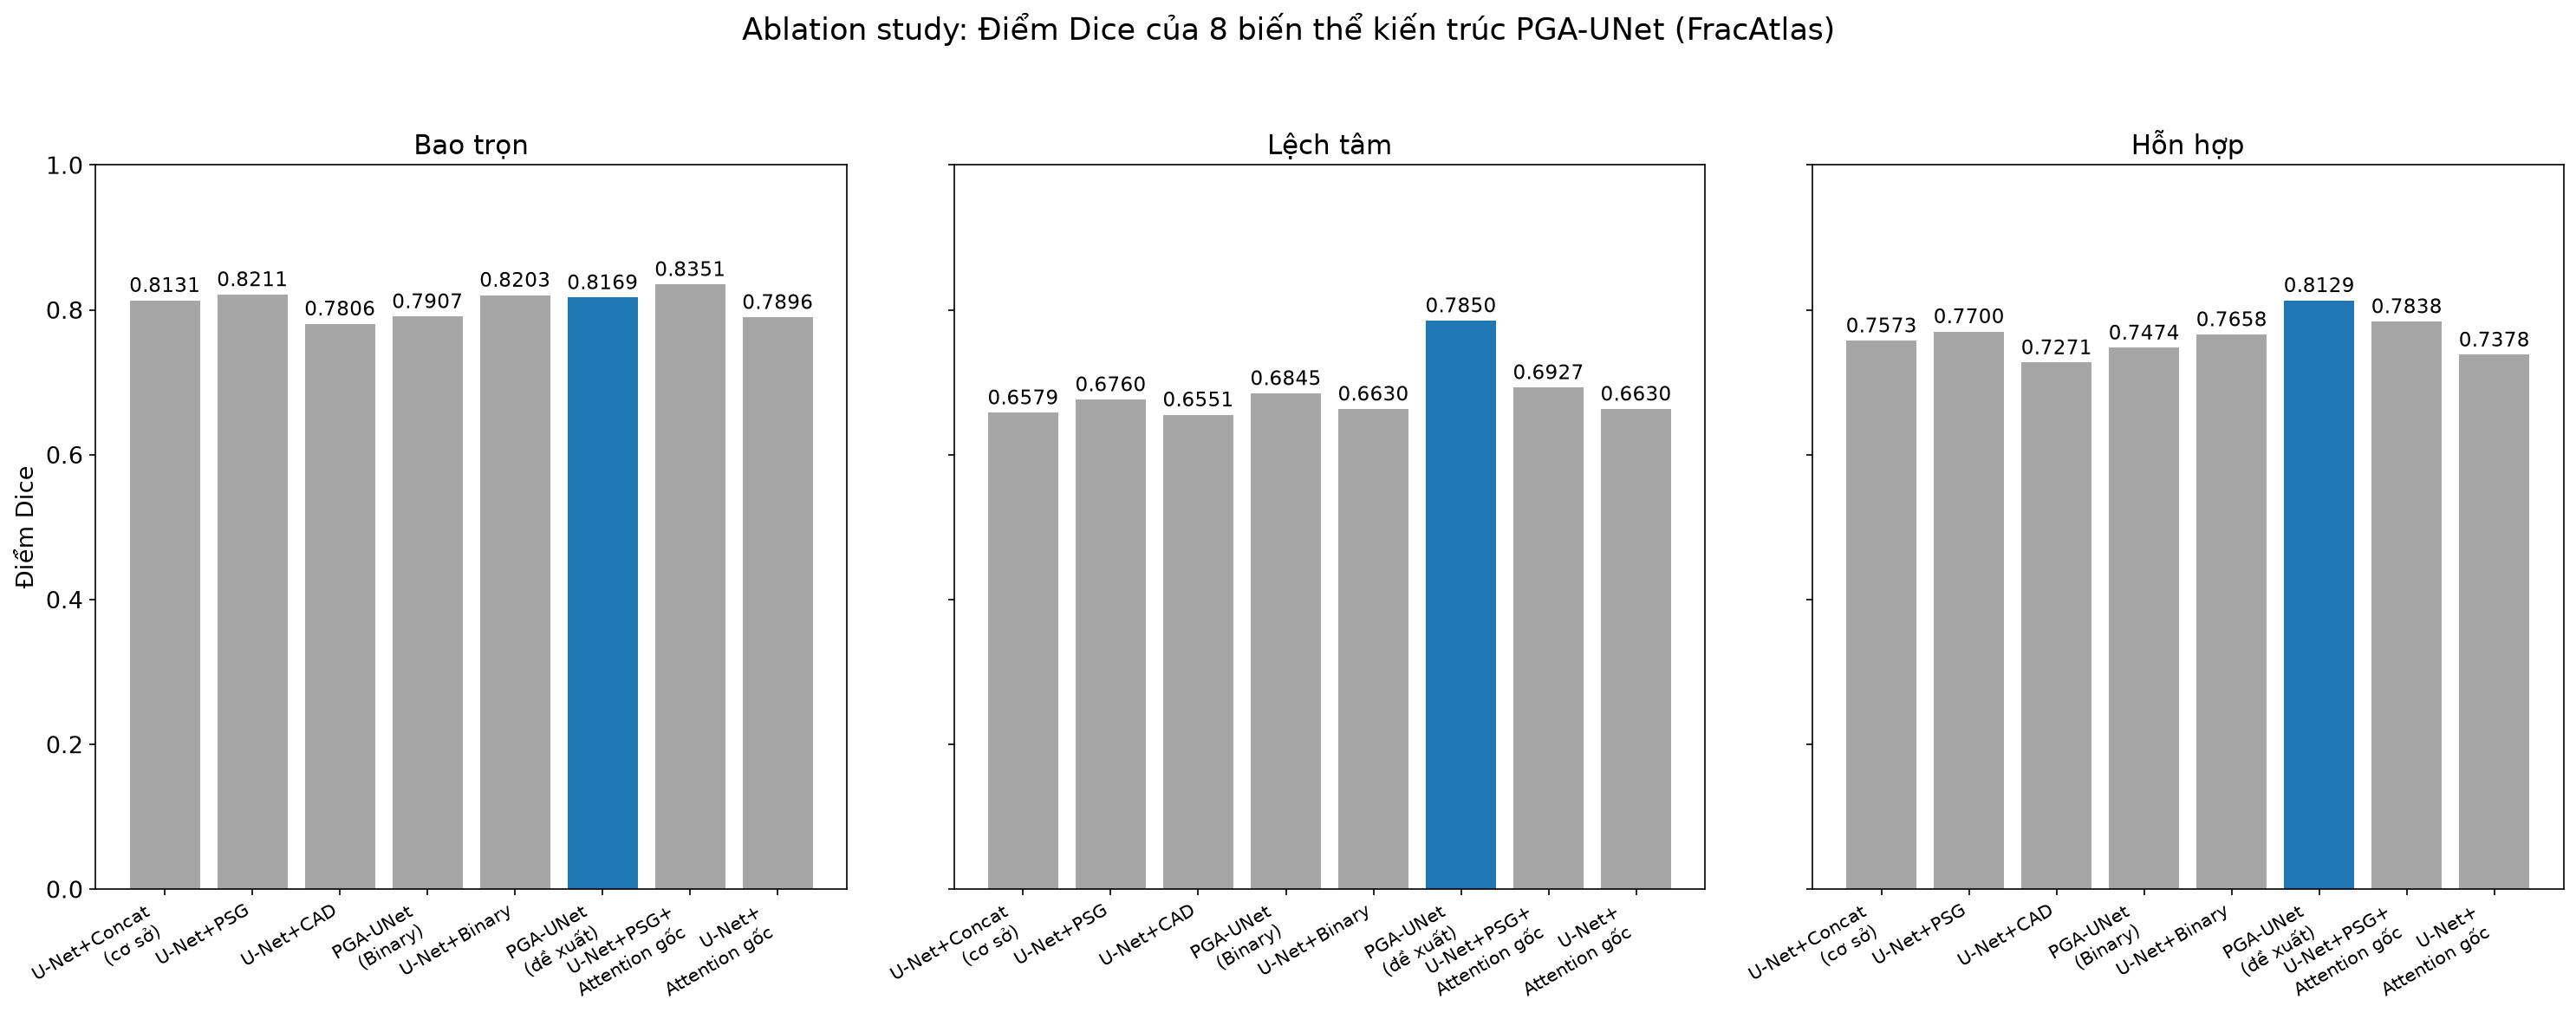
\includegraphics[width=0.95\textwidth]{images/chart_fracatlas_ablation.png}
    \caption{Dice của tám cấu hình trong nghiên cứu loại bỏ thành phần trên FracAtlas. PGA-UNet đạt kết quả cao nhất trong hai kịch bản Lệch tâm và Hỗn hợp.}
    \label{fig:chart_fracatlas_ablation}
\end{figure}

\begin{figure}[H]
    \centering
    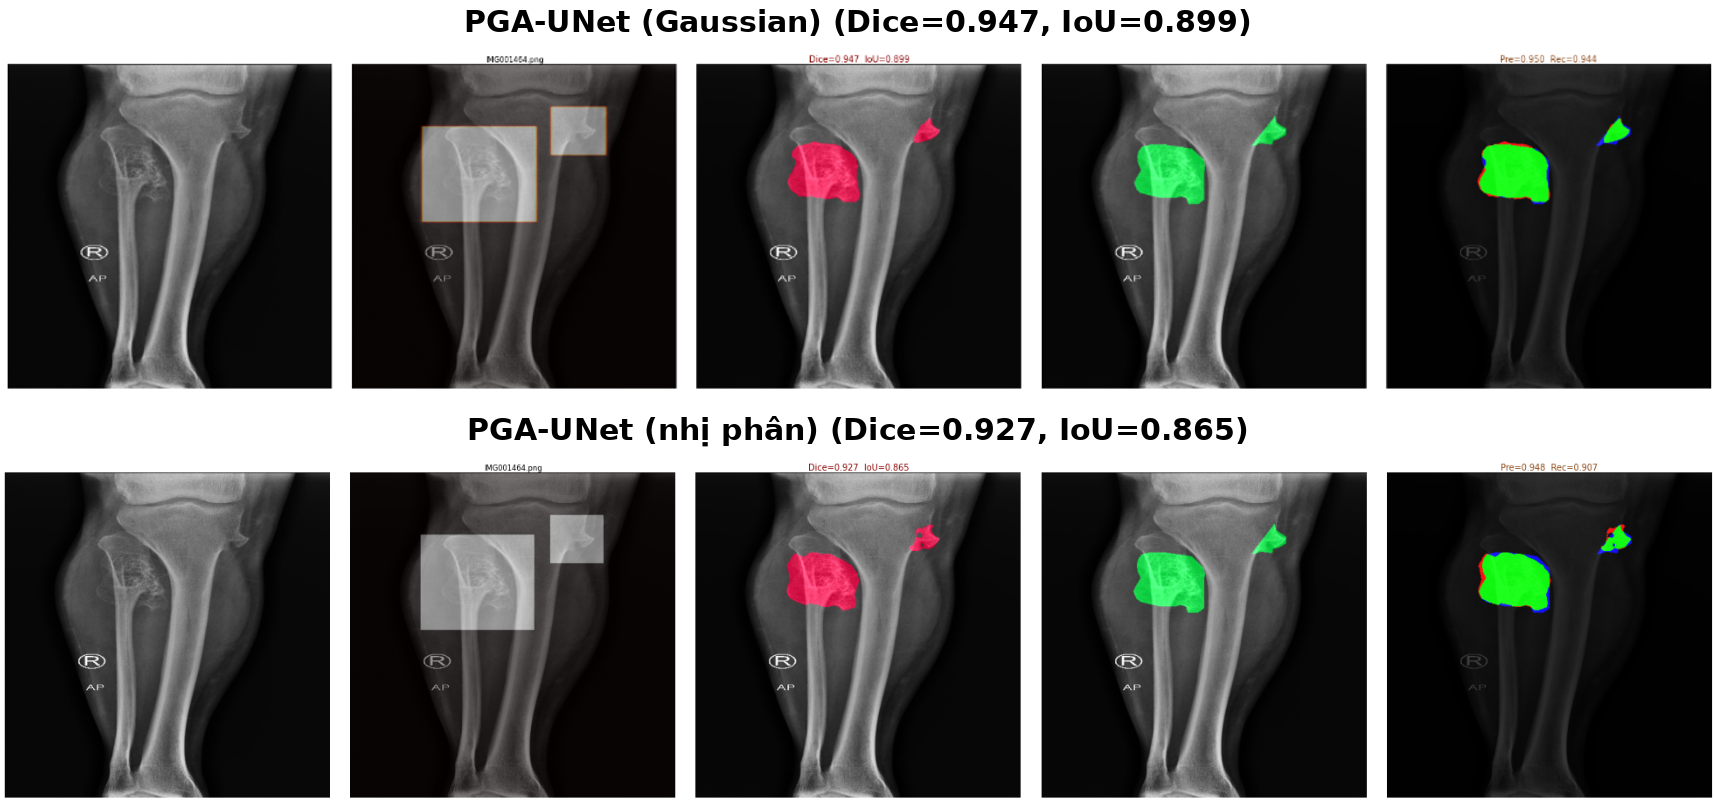
\includegraphics[width=0.65\textwidth]{images/qual_ablation_v4v6_btxrd.png}
    \caption{Minh họa định tính so sánh cấu hình PGA-UNet (Gaussian) với cấu hình dùng câu nhắc nhị phân trên BTXRD, tương ứng hai hàng cuối của Bảng~\ref{tab:ablation_arch}.}
    \label{fig:qual_ablation_v6v7_btxrd}
\end{figure}


\begin{figure}[H]
    \centering
    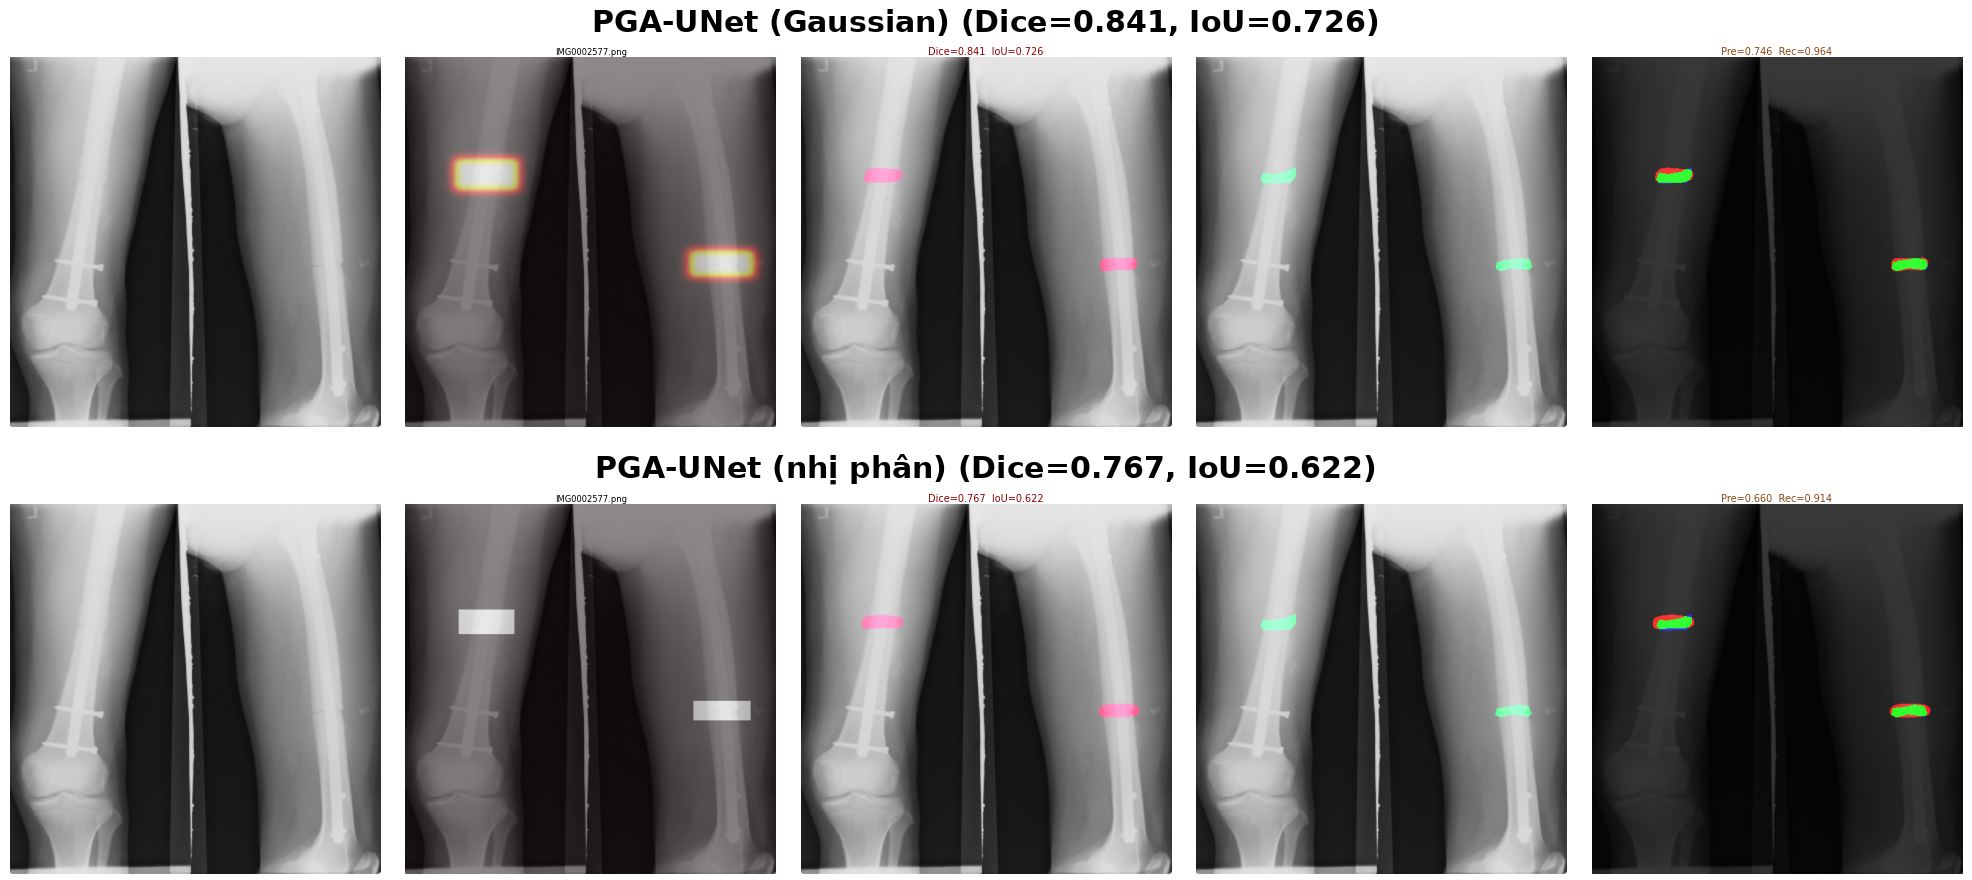
\includegraphics[width=0.65\textwidth]{images/qual_ablation_v4v6_fracatlas.png}
    \caption{Minh họa định tính so sánh cấu hình PGA-UNet (Gaussian) với cấu hình dùng câu nhắc nhị phân trên FracAtlas, tương ứng hai hàng cuối của Bảng~\ref{tab:fracatlas_ablation_arch}.}
    \label{fig:qual_ablation_v6v7_fracatlas}
\end{figure}

Các nhận xét trên dựa vào sự chênh lệch Dice trung bình. Kiểm định Wilcoxon signed-rank trên Dice bắt cặp theo từng ảnh và phần đối chiếu chính thức giữa BTXRD với FracAtlas được trình bày tại Mục~\ref{subsec:conclusion_arch}.

% ------------------------------------------------------------
\subsection{Độ ổn định qua kiểm chứng chéo ngẫu nhiên lặp lại}
\label{subsec:cross_validation_fa}
% ------------------------------------------------------------

PGA-UNet ở độ phân giải $512\times512$ được đánh giá trên FracAtlas bằng cùng phương pháp kiểm chứng chéo ngẫu nhiên lặp lại 4 lần đã áp dụng cho BTXRD tại Mục~\ref{subsec:cross_validation}. Số mẫu đa giác ở mỗi lần dao động nhẹ từ 89 đến 95 vì số vùng gãy trên mỗi ảnh không giống nhau.

Bảng~\ref{tab:cross_validation_fa_per_fold} trình bày Dice của từng lần trong ba kịch bản câu nhắc. Kết quả trung bình trên bốn lần đối với đầy đủ sáu chỉ số được tổng hợp trong Bảng~\ref{tab:cross_validation_fa}.

\begin{table}[H]
    \centering
    \caption{Dice của PGA-UNet trong kiểm chứng chéo ngẫu nhiên lặp lại 4 lần trên FracAtlas}
    \vspace{0.2cm}
    \label{tab:cross_validation_fa_per_fold}
    \renewcommand{\arraystretch}{1.3}
    \resizebox{\textwidth}{!}{%
    \begin{tabular}{|c|c|c|c|c|}
        \hline
        \textbf{Lần}
        & \textbf{Bao trọn↑}
        & \textbf{Lệch tâm↑}
        & \textbf{Hỗn hợp↑} \\
        \hline
        1 & 0.8127 & 0.8025 & 0.8060 \\
        \hline
        2 & 0.8026 & 0.7862 & 0.7981 \\
        \hline
        3 & 0.8200 & 0.7930 & 0.8161 \\
        \hline
        4 & 0.8222 & 0.7798 & 0.8082 \\
        \hline
        \textbf{Trung bình $\pm$ độ lệch chuẩn}
        & $\mathbf{0.8144 \pm 0.0077}$
        & $\mathbf{0.7904 \pm 0.0084}$
        & $\mathbf{0.8071 \pm 0.0064}$ \\
        \hline
    \end{tabular}%
    }
\end{table}

Độ lệch chuẩn Dice dao động từ 0,0064 đến 0,0084, tức là còn thấp hơn so với BTXRD. Kịch bản Lệch tâm vẫn dao động nhiều nhất, điều này phù hợp vì đây là kịch bản có yếu tố ngẫu nhiên ngay trong cách tạo câu nhắc.

\begin{table}[H]
    \centering
    \caption{Kết quả của kiểm chứng chéo ngẫu nhiên lặp lại 4 lần trên FracAtlas}
    \vspace{0.2cm}
    \label{tab:cross_validation_fa}
    \renewcommand{\arraystretch}{1.3}
    \resizebox{\textwidth}{!}{%
    \begin{tabular}{|l|c|c|c|c|c|c|}
        \hline
        \textbf{Kịch bản}
        & \textbf{Dice↑}
        & \textbf{IoU↑}
        & \textbf{Precision↑}
        & \textbf{Recall↑}
        & \textbf{HD95↓ (px)}
        & \textbf{CBL↑} \\
        \hline
        Bao trọn
        & 0.8144 & 0.6955 & 0.7735 & 0.8809 & 8.28 & 0.9541 \\
        \hline
        Lệch tâm
        & 0.7904 & 0.6627 & 0.7589 & 0.8460 & 9.57 & 0.9337 \\
        \hline
        Hỗn hợp (70\% Bao trọn + 30\% Lệch tâm)
        & 0.8071 & 0.6859 & 0.7671 & 0.8723 & 8.84 & 0.9476 \\
        \hline
    \end{tabular}%
    }
\end{table}

So với kết quả trên tập kiểm thử chính tại Bảng~\ref{tab:fracatlas_pga_full}, Dice trung bình chỉ chênh 0,0025 ở Bao trọn, 0,0054 ở Lệch tâm và 0,0058 ở Hỗn hợp. Điều này cho thấy độ ổn định trước cách chia dữ liệu không phải đặc thù riêng của tập BTXRD.

% ------------------------------------------------------------
\subsection{Phân tích theo đặc tính tổn thương}
\label{subsec:fracatlas_subcat}
% ------------------------------------------------------------

Tương tự Mục~\ref{subsec:subcategory}, mục này phân tích hiệu năng của PGA-UNet trên FracAtlas theo các nhóm ảnh có đặc điểm tổn thương khác nhau. Ba phép so sánh được thực hiện: so sánh với U-Net trên các ảnh mà U-Net hoạt động tốt hoặc kém; so sánh PGA-UNet với SAM-Med2D ở cùng độ phân giải $256\times256$; và so sánh hai phiên bản PGA-UNet tại $256\times256$ và $512\times512$. Các kết quả phân nhóm chỉ có ý nghĩa mô tả và không thay thế kết quả trung bình trên toàn bộ tập kiểm thử.

\noindent\textbf{So sánh với U-Net theo mức hiệu năng của mô hình cơ sở}\\
Theo cùng tiêu chí phân nhóm đã dùng trên BTXRD (Mục~\ref{subsec:subcategory}), tập kiểm thử FracAtlas được chia thành hai nhóm hậu nghiệm theo chính Dice của U-Net: nhóm có giá trị Dice cao nhất và nhóm có giá trị Dice thấp nhất của U-Net. Do FracAtlas chỉ có \NtestimgFA~ảnh kiểm thử (ít hơn nhiều so với \Ntestimg~ảnh của BTXRD), quy mô mỗi nhóm được điều chỉnh còn N=36 ảnh/nhóm để hai nhóm không chồng lấp nhau ($2\times36=72=$\NtestimgFA).

\begin{table}[H]
    \centering
    \caption{So sánh PGA-UNet với U-Net theo mức hiệu năng của U-Net trên FracAtlas (36 ảnh/nhóm)}
    \label{tab:fracatlas_subcat_baseline}
    \renewcommand{\arraystretch}{1.3}
    \resizebox{\textwidth}{!}{%
    \begin{tabular}{|l|l|c|c|c|c|c|c|}
        \hline
        \textbf{Nhóm}
        & \textbf{Mô hình}
        & \textbf{Dice↑}
        & \textbf{IoU↑}
        & \textbf{Precision↑}
        & \textbf{Recall↑}
        & \textbf{HD95↓ (px)}
        & \textbf{CBL↑} \\
        \hline
        \multirow{2}{*}{U-Net hoạt động tốt}
        & U-Net
        & 0.6532 & 0.5018 & 0.6266 & 0.7500 & 82.10 & 0.7595 \\
        & PGA-UNet
        & \textbf{0.8324}
        & \textbf{0.7179}
        & \textbf{0.7920}
        & \textbf{0.8975}
        & \textbf{8.04}
        & \textbf{0.9600} \\
        \hline
        \multirow{2}{*}{U-Net hoạt động kém}
        & U-Net
        & 0.1130 & 0.0654 & 0.1397 & 0.1784 & 191.54 & 0.1662 \\
        & PGA-UNet
        & \textbf{0.8015}
        & \textbf{0.6726}
        & \textbf{0.7370}
        & \textbf{0.8974}
        & \textbf{6.85}
        & \textbf{0.9493} \\
        \hline
    \end{tabular}%
    }
\end{table}

Xu hướng từ BTXRD (Bảng~\ref{tab:subcat_baseline}) được tái khẳng định trên FracAtlas. Ở nhóm U-Net hoạt động tốt, bản thân U-Net đạt Dice khá (0,6532) vì đây là những ca dễ nhất theo chính đánh giá của U-Net; PGA-UNet vẫn cao hơn 0,1791. Ở nhóm U-Net hoạt động kém, kết quả suy giảm nghiêm trọng (Dice$=0,1130$, HD95$=191,54$ điểm ảnh), trong khi PGA-UNet gần như không đổi so với nhóm U-Net hoạt động tốt (0,8015 so với 0,8324). Tương tự nhận định trên BTXRD, cách phân nhóm này lấy trực tiếp từ kết quả của U-Net nên chỉ mang tính mô tả hai cực hiệu năng của mô hình cơ sở, không phải phân loại theo độ khó của tập dữ liệu.

\begin{figure}[H]
    \centering
    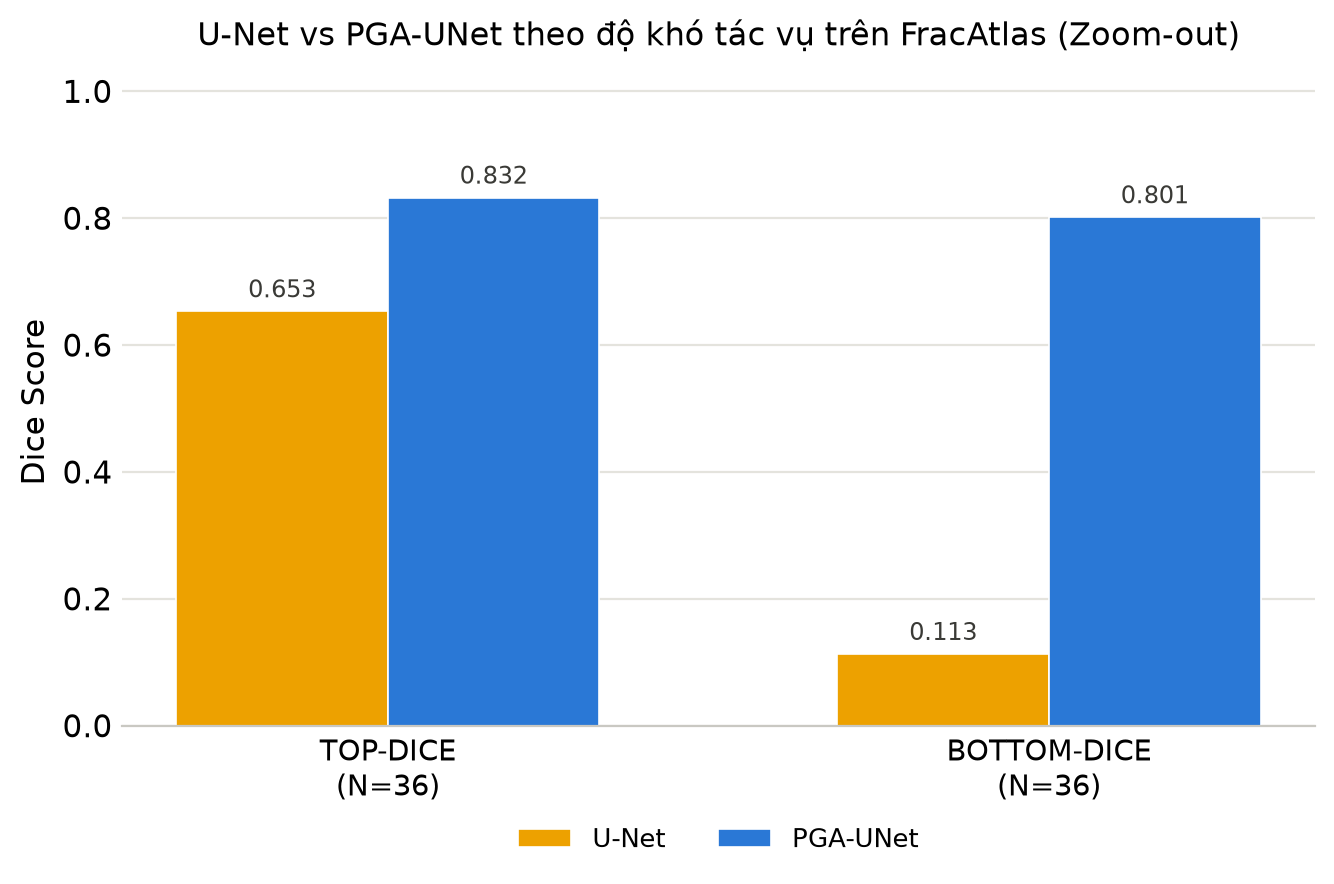
\includegraphics[width=0.7\textwidth, height=9cm, keepaspectratio=false]{images/chart_fracatlas_subcat_baseline.png}
    \caption{Dice của U-Net và PGA-UNet trên nhóm U-Net hoạt động tốt và U-Net hoạt động kém.}
    \label{fig:chart_fracatlas_subcat_baseline}
\end{figure}

Hình~\ref{fig:qual_subcat_baseline_fracatlas} minh họa một ảnh thuộc mỗi nhóm trên tập FracAtlas: ở nhóm U-Net hoạt động tốt, PGA-UNet (Dice$=0,909$) và U-Net (Dice$=0,872$) đều phân đoạn tốt; ở nhóm U-Net hoạt động kém, U-Net không phân đoạn được vùng mục tiêu (Dice$=0,000$) trong khi PGA-UNet vẫn giữ Dice$=0,848$.

\begin{figure}[H]
    \centering
    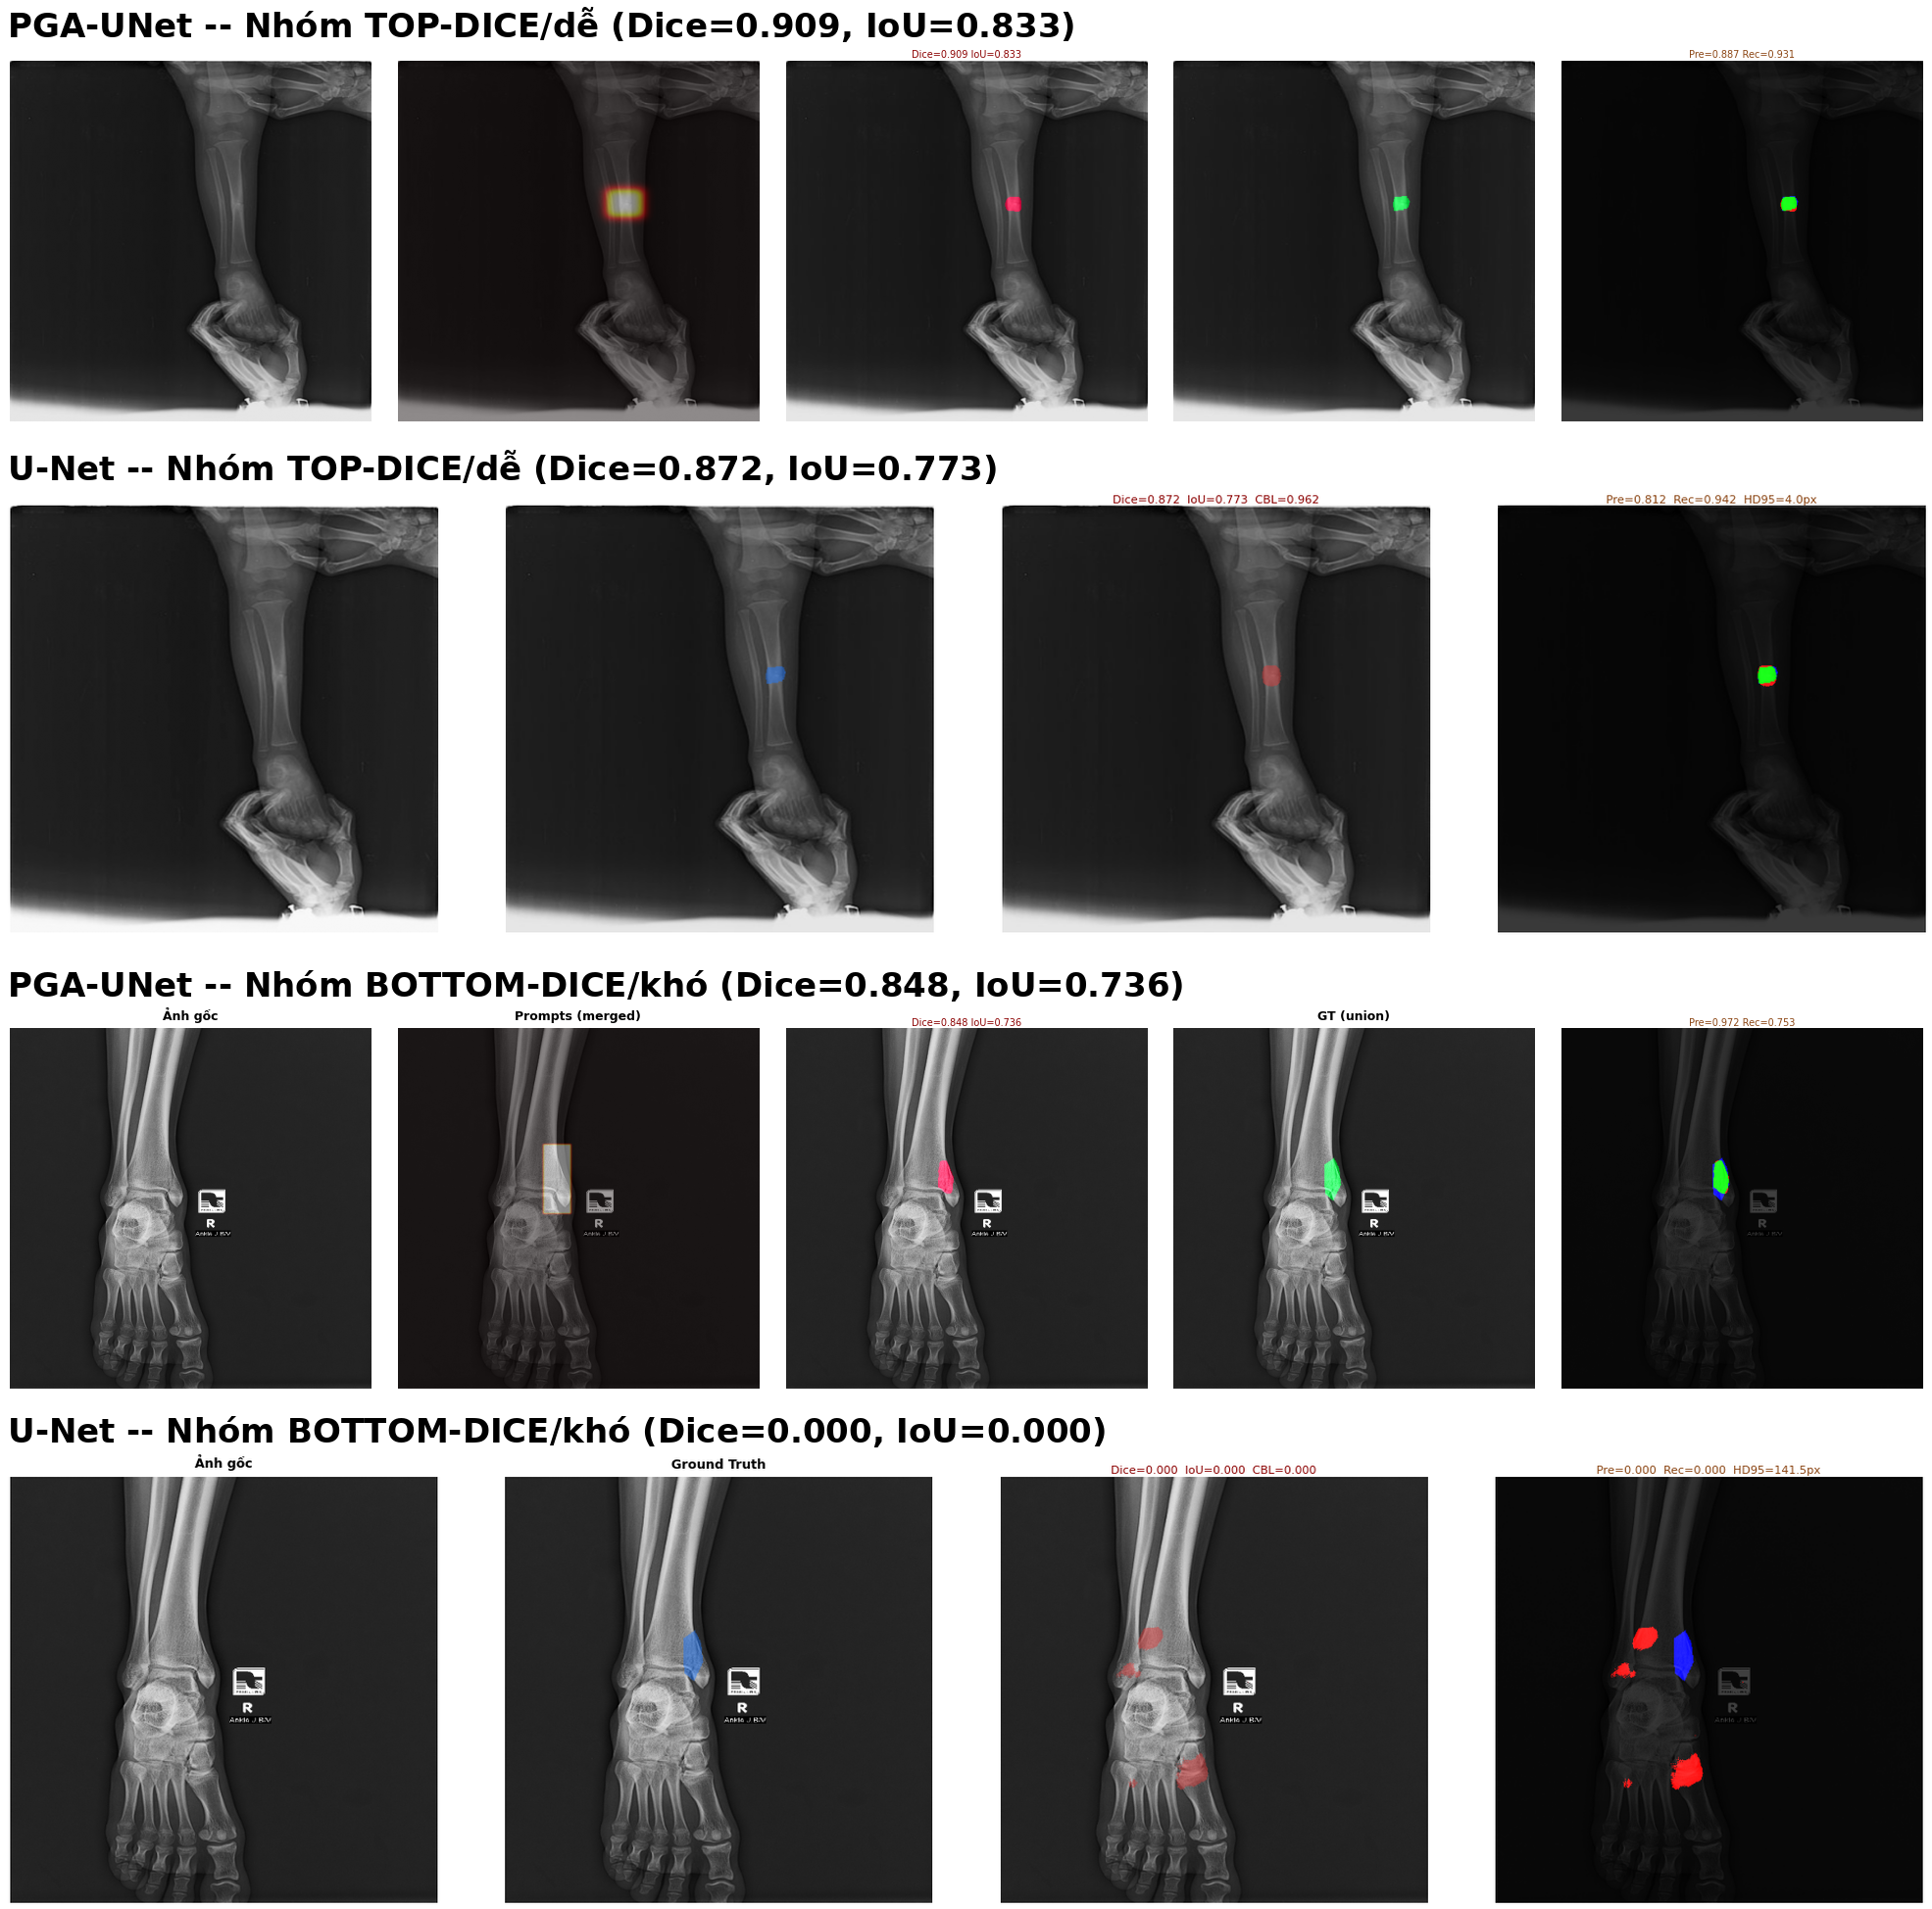
\includegraphics[width=0.65\textwidth]{images/qual_subcat_baseline_fracatlas.png}
    \caption{Kết quả định tính của U-Net và PGA-UNet trên một ảnh thuộc mỗi nhóm hiệu năng của U-Net.}
    \label{fig:qual_subcat_baseline_fracatlas}
\end{figure}

\noindent\textbf{So sánh với SAM-Med2D theo đặc tính tổn thương}\\
Tập kiểm thử FracAtlas được chia thành ba nhóm không chồng lấp, mỗi nhóm gồm 24 ảnh. Nhóm Tổn thương nhỏ gồm các ảnh có tổng diện tích nhãn nhỏ nhất. Trong số ảnh còn lại, 24 ảnh có chỉ số Dice SAM-Med2D thấp nhất được xếp vào nhóm Biên mờ và 24 ảnh còn lại có diện tích tổn thương lớn nhất được xếp vào nhóm Tổn thương rõ.

Tên nhóm Biên mờ được sử dụng như một quy ước mô tả cho những ảnh SAM-Med2D gặp khó khăn. Do nhóm này được xác định dựa trên chính Dice của SAM-Med2D, kết quả thu được chỉ mang tính nhận định sơ bộ và không được xem là đánh giá khách quan về độ khó của tổn thương.

Để bảo đảm so sánh công bằng, PGA-UNet và SAM-Med2D trước hết được đối chiếu ở cùng độ phân giải $256\times256$, trên cùng nhóm ảnh và cùng hộp giới hạn. Kết quả được trình bày trong Bảng~\ref{tab:fracatlas_subcat_sam_256}.

\begin{table}[H]
    \centering
    \caption{So sánh PGA-UNet với SAM-Med2D theo đặc tính tổn thương ở cùng độ phân giải $256\times256$ trên FracAtlas (Bao trọn, 24 ảnh/nhóm)}
    \label{tab:fracatlas_subcat_sam_256}
    \renewcommand{\arraystretch}{1.3}
    \resizebox{\textwidth}{!}{%
    \begin{tabular}{|l|l|c|c|c|c|c|c|}
        \hline
        \textbf{Nhóm}
        & \textbf{Mô hình}
        & \textbf{Dice↑}
        & \textbf{IoU↑}
        & \textbf{Precision↑}
        & \textbf{Recall↑}
        & \textbf{HD95↓ (px)}
        & \textbf{CBL↑} \\
        \hline
        \multirow{2}{*}{Tổn thương nhỏ}
        & SAM-Med2D ($256\times256$)
        & 0.4395 & 0.3141 & \textbf{0.7793} & 0.3507 & 30.94 & 0.8210 \\
        & PGA-UNet ($256\times256$)
        & \textbf{0.7584}
        & \textbf{0.6178}
        & 0.6652
        & \textbf{0.9006}
        & \textbf{6.04}
        & \textbf{0.9125} \\
        \hline
        \multirow{2}{*}{Biên mờ}
        & SAM-Med2D ($256\times256$)
        & 0.5787 & 0.4132 & \textbf{0.7814} & 0.4953 & 14.80 & 0.9005 \\
        & PGA-UNet ($256\times256$)
        & \textbf{0.7926}
        & \textbf{0.6627}
        & 0.7118
        & \textbf{0.9060}
        & \textbf{9.41}
        & \textbf{0.9566} \\
        \hline
        \multirow{2}{*}{Tổn thương rõ}
        & SAM-Med2D ($256\times256$)
        & 0.7677 & 0.6253 & \textbf{0.8451} & 0.7178 & 9.86 & 0.9373 \\
        & PGA-UNet ($256\times256$)
        & \textbf{0.8358}
        & \textbf{0.7213}
        & 0.8105
        & \textbf{0.8801}
        & \textbf{8.17}
        & \textbf{0.9563} \\
        \hline
    \end{tabular}%
    }
\end{table}

Ở cùng độ phân giải, PGA-UNet đạt Dice cao hơn SAM-Med2D trong cả ba nhóm. Mức chênh lệch xấp xỉ 0,319 ở Tổn thương nhỏ, 0,214 ở Biên mờ và 0,068 ở Tổn thương rõ. Khoảng cách giảm dần khi tổn thương có kích thước lớn và hình thái rõ hơn.

Ở nhóm Tổn thương nhỏ, PGA-UNet đạt Recall 0,9006, trong khi SAM-Med2D chỉ đạt 0,3507. Tuy nhiên, Precision của SAM-Med2D lại cao hơn, đạt 0,7793 so với 0,6652. Xu hướng tương tự xuất hiện ở hai nhóm còn lại: SAM-Med2D có Precision cao hơn, còn PGA-UNet đạt Recall, Dice và CBL cao hơn. Có thể hiểu là SAM-Med2D dự đoán thận trọng hơn, còn PGA-UNet bao phủ được nhiều điểm ảnh tổn thương hơn.

Ở nhóm Tổn thương rõ, khoảng cách Dice thu hẹp còn khoảng 0,068, tức là kết quả hai mô hình gần nhau hơn khi vùng tổn thương dễ xác định. Riêng kết quả ở nhóm Biên mờ cần được diễn giải thận trọng vì nhóm này được lựa chọn dựa trên Dice thấp của SAM-Med2D.

\begin{figure}[H]
    \centering
    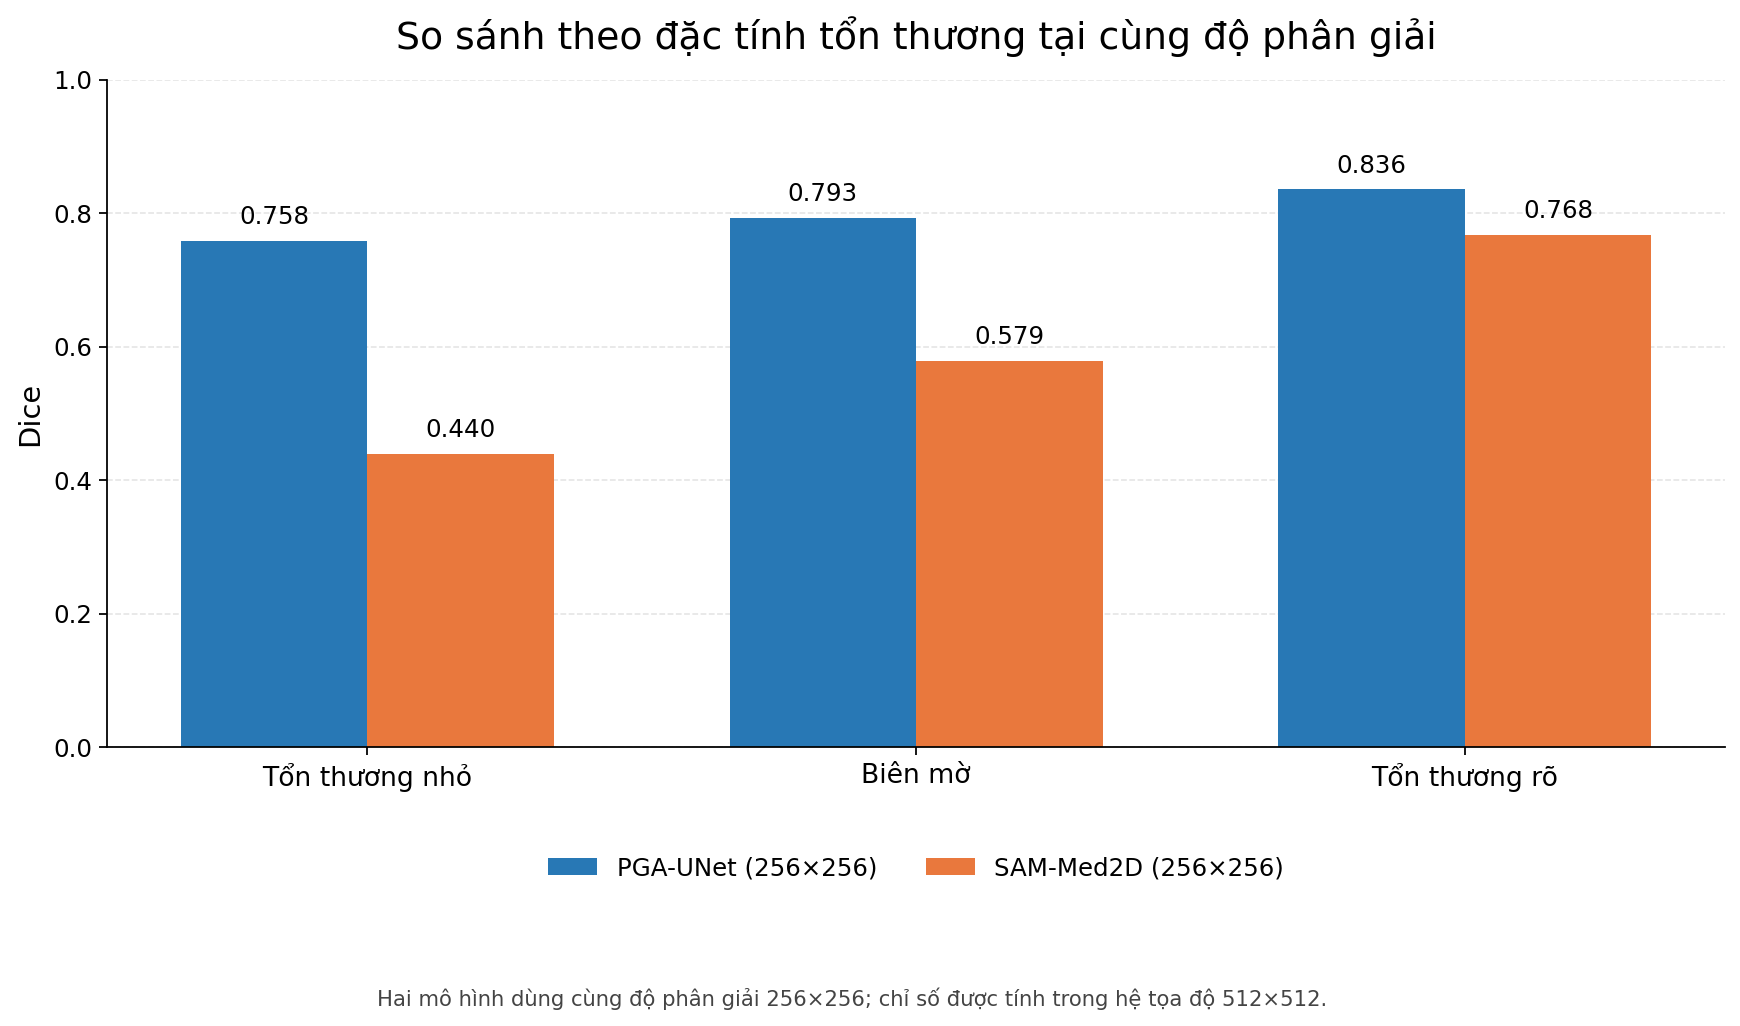
\includegraphics[width=0.9\textwidth]{images/chart_fracatlas_pga256_sam256.png}
    \caption{So sánh Dice của PGA-UNet và SAM-Med2D theo đặc tính tổn thương ở cùng độ phân giải $256\times256$ trên FracAtlas.}
    \label{fig:chart_fracatlas_pga256_sam256}
\end{figure}

\begin{figure}[H]
    \centering
    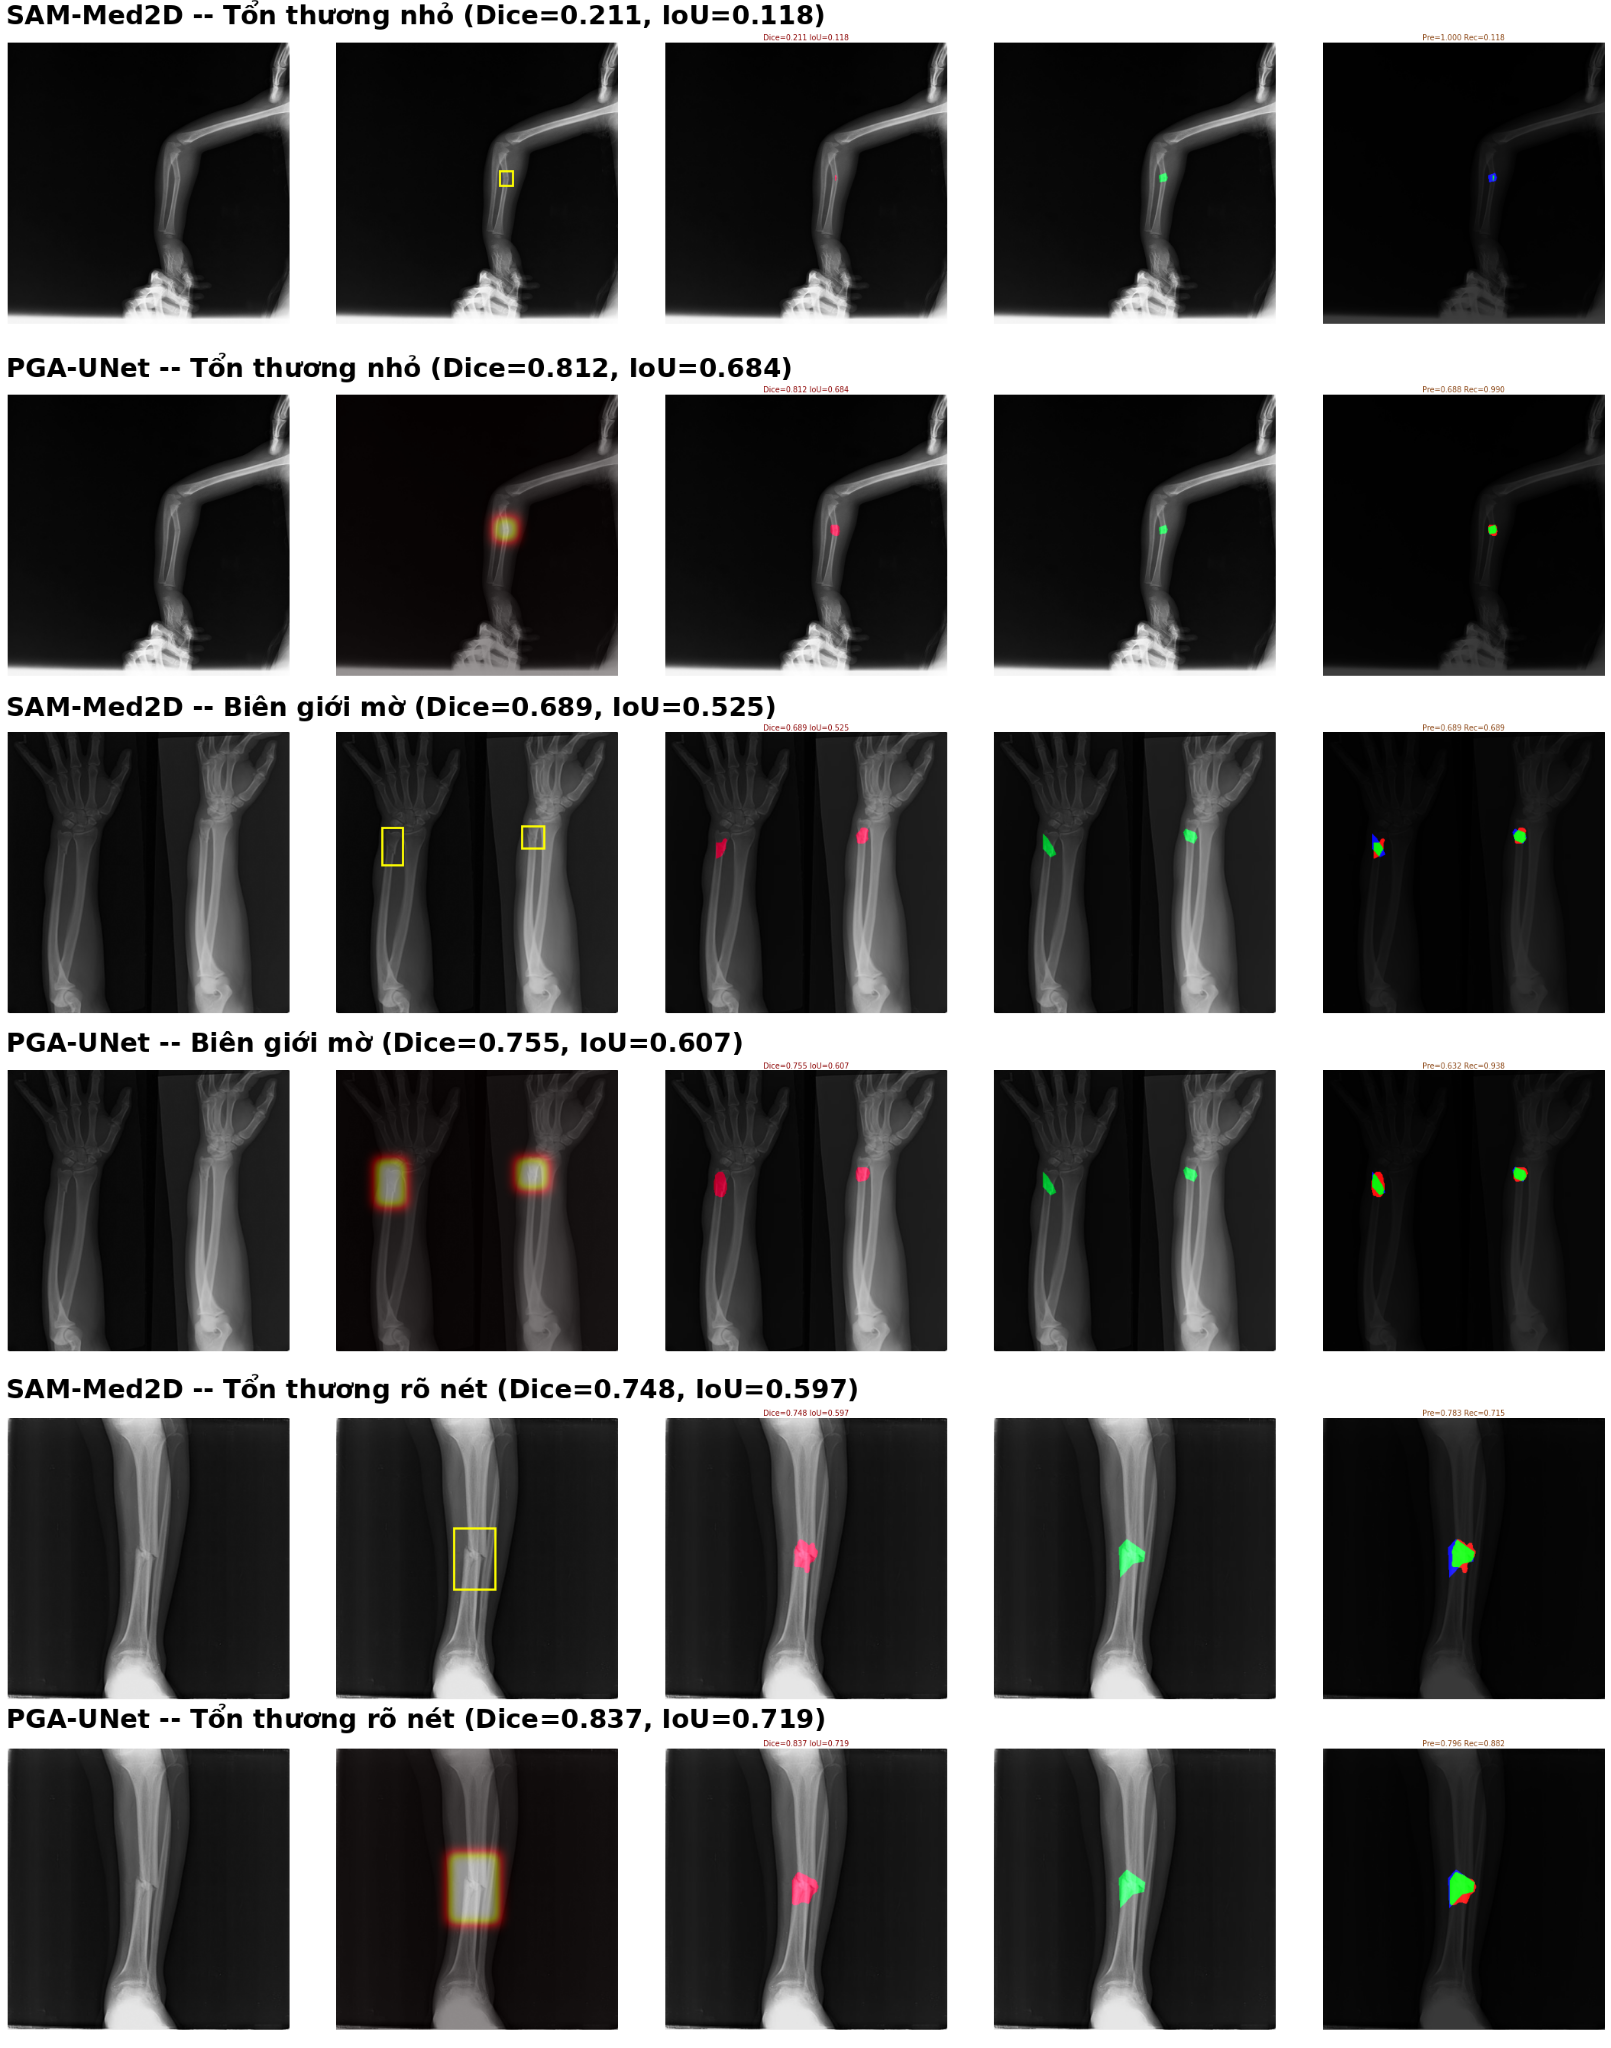
\includegraphics[width=0.9\textwidth]{images/qual_subcat_sam_fracatlas.png}
    \caption{Kết quả định tính của SAM-Med2D và PGA-UNet trên các ảnh đại diện thuộc ba nhóm đặc tính tổn thương trên FracAtlas.}
    \label{fig:qual_subcat_sam_fracatlas}
\end{figure}

\noindent\textbf{Ảnh hưởng của độ phân giải theo đặc tính tổn thương}\\
Hai phiên bản PGA-UNet được tiếp tục đối chiếu trên cùng ba nhóm ảnh để xác định ảnh hưởng của việc tăng độ phân giải từ $256\times256$ lên $512\times512$. Ngoài độ phân giải và điểm lưu trọng số tương ứng, các điều kiện đánh giá được giữ nguyên.

\begin{table}[H]
    \centering
    \caption{Ảnh hưởng của độ phân giải đối với PGA-UNet theo đặc tính tổn thương trên FracAtlas (Bao trọn, 24 ảnh/nhóm)}
    \label{tab:fracatlas_subcat_pga_resolution}
    \renewcommand{\arraystretch}{1.3}
    \resizebox{\textwidth}{!}{%
    \begin{tabular}{|l|l|c|c|c|c|c|c|}
        \hline
        \textbf{Nhóm}
        & \textbf{Độ phân giải}
        & \textbf{Dice↑}
        & \textbf{IoU↑}
        & \textbf{Precision↑}
        & \textbf{Recall↑}
        & \textbf{HD95↓ (px)}
        & \textbf{CBL↑} \\
        \hline
        \multirow{2}{*}{Tổn thương nhỏ}
        & $256\times256$
        & 0.7584 & 0.6178 & 0.6652 & 0.9006 & 6.04 & 0.9125 \\
        & $512\times512$
        & \textbf{0.8028}
        & \textbf{0.6756}
        & \textbf{0.7269}
        & \textbf{0.9150}
        & 5.05
        & \textbf{0.9400} \\
        \hline
        \multirow{2}{*}{Biên mờ}
        & $256\times256$
        & 0.7926 & 0.6627 & 0.7118 & \textbf{0.9060} & 9.41 & \textbf{0.9566} \\
        & $512\times512$
        & \textbf{0.8039}
        & \textbf{0.6775}
        & \textbf{0.7439}
        & 0.8925
        & 9.29
        & 0.9552 \\
        \hline
        \multirow{2}{*}{Tổn thương rõ}
        & $256\times256$
        & 0.8358 & 0.7213 & 0.8105 & \textbf{0.8801} & 8.17 & 0.9563 \\
        & $512\times512$
        & \textbf{0.8404}
        & \textbf{0.7280}
        & \textbf{0.8203}
        & 0.8786
        & 8.09
        & \textbf{0.9626} \\
        \hline
    \end{tabular}%
    }
\end{table}

Việc tăng độ phân giải giúp cải thiện Dice trên cả ba nhóm, nhưng mức tăng lớn nhất xuất hiện ở Tổn thương nhỏ. Dice của nhóm này tăng 0,0444, từ 0,7584 lên 0,8028; Precision tăng 0,0617 và CBL tăng 0,0275. Có thể thấy tổn thương nhỏ cải thiện rõ nhất từ việc giữ được nhiều chi tiết không gian hơn ở đầu vào.

Ở nhóm Biên mờ, Dice chỉ tăng 0,0113; ở nhóm Tổn thương rõ, mức tăng còn 0,0046. Hai nhóm này ít nhạy với độ phân giải hơn Tổn thương nhỏ. Recall của phiên bản 256 cao hơn không nhiều trong hai nhóm này, trong khi phiên bản 512 đạt Dice, IoU và Precision cao hơn.

\begin{figure}[H]
    \centering
    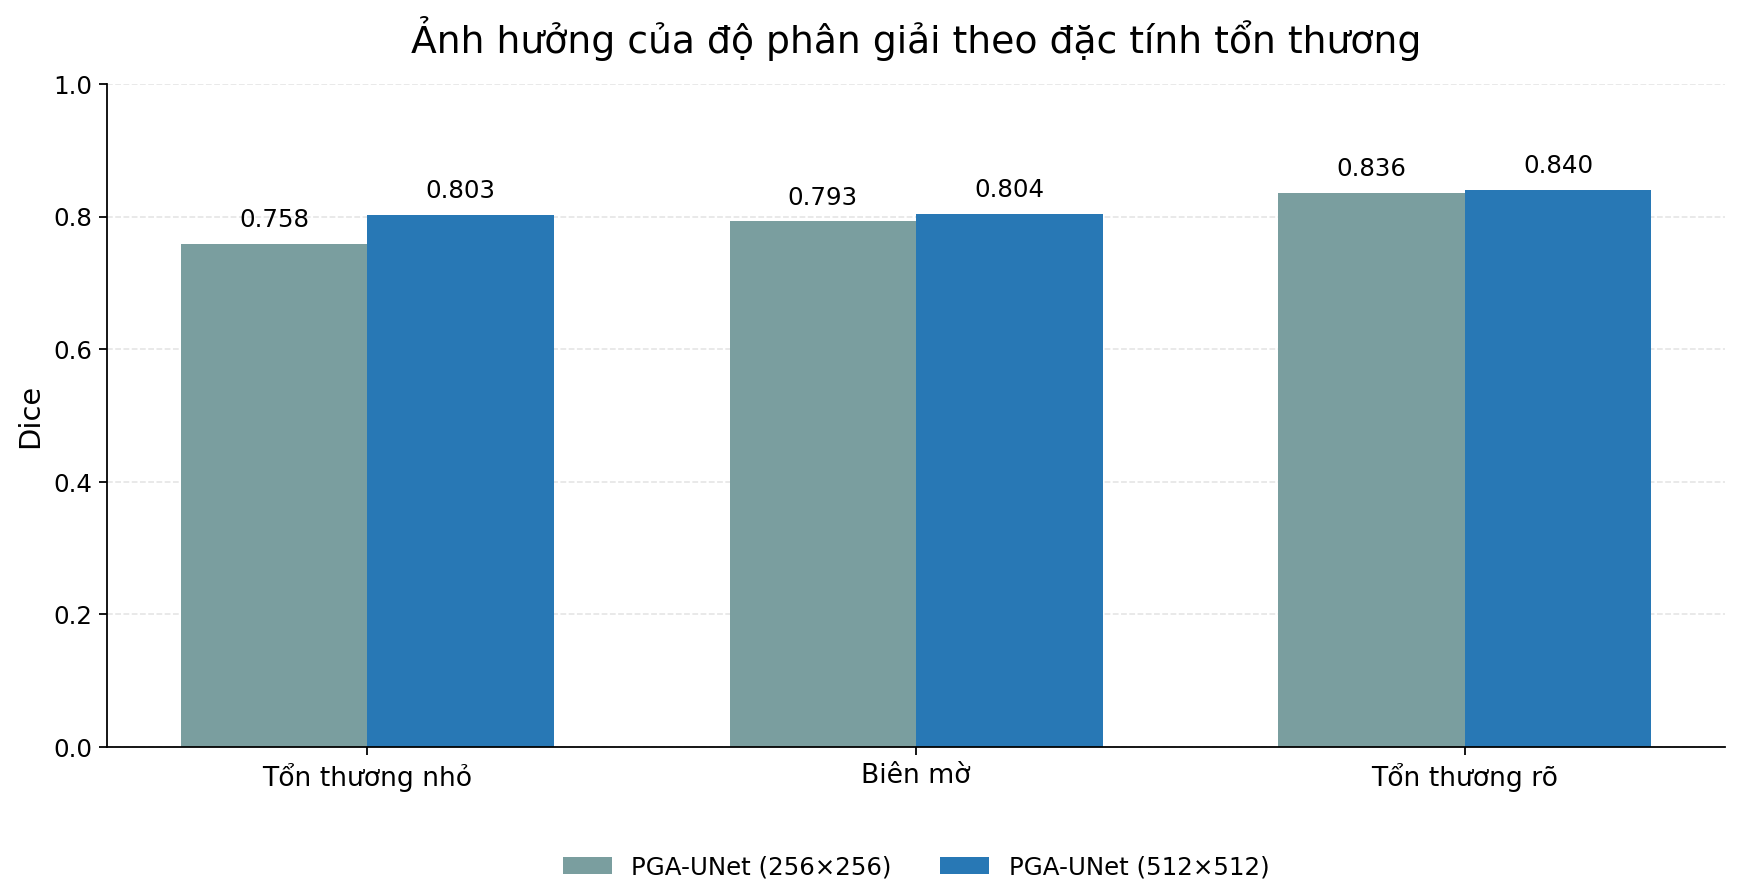
\includegraphics[width=0.9\textwidth]{images/chart_fracatlas_pga_resolution.png}
    \caption{Ảnh hưởng của độ phân giải đến Dice của PGA-UNet theo ba nhóm đặc tính tổn thương trên FracAtlas.}
    \label{fig:chart_fracatlas_pga_resolution}
\end{figure}

\noindent\textbf{Kết luận}\\
Khi kiểm soát độ phân giải ở $256\times256$, PGA-UNet vẫn đạt Dice cao hơn SAM-Med2D trên cả ba nhóm, đặc biệt ở Tổn thương nhỏ và nhóm ảnh SAM-Med2D gặp khó khăn. Khi thay đổi độ phân giải của PGA-UNet, nhóm Tổn thương nhỏ tiếp tục nhận được mức cải thiện lớn hơn. Hai kết quả cho thấy ưu thế của PGA-UNet trên tổn thương nhỏ không chỉ đến từ việc sử dụng ảnh $512\times512$, mặc dù độ phân giải cao vẫn giúp cải thiện thêm hiệu năng.

% ------------------------------------------------------------
\section{Kết luận đóng góp kiến trúc trên hai miền dữ liệu}
\label{subsec:conclusion_arch}
% ------------------------------------------------------------

Các nghiên cứu loại bỏ thành phần trên BTXRD tại Mục~\ref{subsec:ablation_arch} và FracAtlas tại Mục~\ref{subsec:fracatlas_ablation} trước hết dựa trên chênh lệch Dice trung bình. Để đánh giá độ tin cậy của các chênh lệch này ở cấp độ ảnh, sáu cặp cấu hình tương ứng được kiểm tra bằng kiểm định thống kê Wilcoxon trên Dice bắt cặp theo từng ảnh.

Kiểm định được thực hiện riêng trên BTXRD và FracAtlas trong ba kịch bản câu nhắc. Bảng~\ref{tab:wilcoxon_ablation} báo cáo các giá trị $p$ chưa hiệu chỉnh cho việc thực hiện nhiều phép so sánh. Vì vậy, các kết quả có $p<0{,}001$ được xem là bằng chứng mạnh hơn, còn các giá trị gần ngưỡng $0{,}05$ chỉ được diễn giải theo hướng thăm dò.

\begin{table}[H]
    \centering
    \caption{Kiểm định Wilcoxon cho sáu cặp cấu hình trên BTXRD và FracAtlas. $\Delta$Dice được tính bằng Dice của cấu hình thứ nhất trừ cấu hình thứ hai; các giá trị $p$ chưa được hiệu chỉnh cho so sánh nhiều lần}
    \label{tab:wilcoxon_ablation}
    \renewcommand{\arraystretch}{1.2}
    \resizebox{\textwidth}{!}{%
    \begin{tabular}{|p{7.5cm}|l|c|c|c|c|}
        \hline
        \textbf{Cặp cấu hình}
        & \textbf{Kịch bản}
        & \textbf{$\Delta$Dice BTXRD}
        & \textbf{$p$ BTXRD}
        & \textbf{$\Delta$Dice FracAtlas}
        & \textbf{$p$ FracAtlas} \\
        \hline

        \multirow{3}{5.6cm}{U-Net + Cổng chú ý nguyên bản $-$ U-Net+Concat(Gaussian)}
        & Bao trọn & $-0.0024$ & 0,255 & $-0.0235$ & $<0{,}001$ \\
        & Lệch tâm & $-0.0050$ & 0,607 & $+0.0050$ & 0,255 \\
        & Hỗn hợp & $-0.0023$ & 0,395 & $-0.0195$ & $<0{,}001$ \\
        \hline

        \multirow{3}{5.6cm}{U-Net + CAD $-$ U-Net+Cổng chú ý nguyên bản}
        & Bao trọn & $+0.0122$ & $<0{,}001$ & $-0.0089$ & 0,025 \\
        & Lệch tâm & $+0.0092$ & 0,152 & $-0.0079$ & 0,141 \\
        & Hỗn hợp & $+0.0098$ & 0,003 & $-0.0107$ & 0,023 \\
        \hline

        \multirow{3}{5.6cm}{U-Net + PSG + Cổng chú ý nguyên bản $-$ U-Net + PSG}
        & Bao trọn & $+0.0007$ & 0,129 & $+0.0140$ & 0,009 \\
        & Lệch tâm & $-0.0030$ & 0,376 & $+0.0167$ & 0,005 \\
        & Hỗn hợp & $+0.0011$ & 0,074 & $+0.0138$ & 0,002 \\
        \hline

        \multirow{3}{5.6cm}{PGA - UNet (Gaussian) $-$ U-Net + PSG + Cổng chú ý nguyên bản}
        & Bao trọn & $-0.0073$ & 0,025 & $-0.0182$ & $<0{,}001$ \\
        & Lệch tâm & $\mathbf{+0.1065}$ & $\mathbf{<0{,}001}$ & $\mathbf{+0.0924}$ & $\mathbf{<0{,}001}$ \\
        & Hỗn hợp & $+0.0388$ & 0,001 & $+0.0291$ & 0,161 \\
        \hline

        \multirow{3}{5.6cm}{U-Net + Concat (Gaussian) $-$ U-Net + Concat (nhị phân)}
        & Bao trọn & $-0.0018$ & 0,896 & $-0.0072$ & 0,007 \\
        & Lệch tâm & $+0.0052$ & 0,013 & $-0.0050$ & 0,284 \\
        & Hỗn hợp & $+0.0015$ & 0,226 & $-0.0085$ & 0,006 \\
        \hline

        \multirow{3}{5.6cm}{PGA-UNet (Gaussian) $-$ PGA-UNet (nhị phân)}
        & Bao trọn & $-0.0173$ & $<0{,}001$ & $+0.0262$ & $<0{,}001$ \\
        & Lệch tâm & $\mathbf{+0.0990}$ & $\mathbf{<0{,}001}$ & $\mathbf{+0.1005}$ & $\mathbf{<0{,}001}$ \\
        & Hỗn hợp & $+0.0293$ & 0,012 & $+0.0655$ & $<0{,}001$ \\
        \hline
    \end{tabular}%
    }
\end{table}

\noindent\textbf{Vai trò của CAD đối với khả năng duy trì hiệu năng dưới sai lệch câu nhắc trong phạm vi bài toán}\\
Kết quả nhất quán nhất giữa hai bộ dữ liệu xuất hiện khi so sánh PGA-UNet với cấu hình dùng PSG và cổng chú ý nguyên bản. Trong kịch bản Lệch tâm, việc thay cổng chú ý nguyên bản bằng CAD làm Dice tăng 0,1065 trên BTXRD và 0,0924 trên FracAtlas; cả hai phép kiểm định đều đạt $p<0{,}001$.

Ở kịch bản Hỗn hợp, mức tăng đạt 0,0388 trên BTXRD và 0,0291 trên FracAtlas, nhưng chỉ kết quả BTXRD đạt giá trị $p$ dưới 0,05. Trong kịch bản Bao trọn, PGA-UNet thấp hơn cấu hình dùng cổng chú ý nguyên bản 0,0073 trên BTXRD và 0,0182 trên FracAtlas.

Như vậy, bằng chứng mạnh và nhất quán nhất của CAD nằm ở kịch bản Lệch tâm. CAD không tối đa hóa Dice khi hộp giới hạn hoàn toàn lý tưởng, nhưng giúp mô hình duy trì hiệu năng tốt hơn khi vị trí câu nhắc bị sai lệch. Kết quả này phù hợp với mục tiêu thiết kế PGA-UNet là tăng mức ổn định dưới sai số hộp giới hạn đã được mô phỏng trong thực nghiệm.

\noindent\textbf{Vai trò của bản đồ nhiệt Gaussian}\\
Khi câu nhắc chỉ được nối vào đầu vào, chênh lệch Dice giữa Gaussian và mặt nạ nhị phân đều nhỏ hơn 0,01 và không nhất quán về chiều giữa hai bộ dữ liệu. Điều này cho thấy chỉ riêng cách biểu diễn câu nhắc chưa đủ để tạo khác biệt lớn nếu kiến trúc không có cơ chế khai thác câu nhắc ở nhiều tầng.

Trong cấu hình đầy đủ PSG+CAD, Gaussian tạo ra mức cải thiện rõ rệt ở các kịch bản có câu nhắc lệch. So với PGA-UNet dùng câu nhắc nhị phân, phiên bản Gaussian tăng 0,0990 Dice trên BTXRD và 0,1005 trên FracAtlas ở kịch bản Lệch tâm, với $p<0{,}001$ trên cả hai bộ dữ liệu. Trong kịch bản Hỗn hợp, mức tăng tương ứng là 0,0293 và 0,0655.

Riêng kịch bản Bao trọn có kết quả khác nhau giữa hai miền: Gaussian thấp hơn nhị phân 0,0173 trên BTXRD nhưng cao hơn 0,0262 trên FracAtlas. Vì vậy, đóng góp nhất quán của Gaussian không nằm ở kịch bản lý tưởng mà ở khả năng hỗ trợ mô hình khi câu nhắc bị lệch, đặc biệt khi được kết hợp với PSG và CAD.

\noindent\textbf{Đóng góp riêng lẻ của PSG và cơ chế chú ý}\\
Các thành phần riêng lẻ có mức ảnh hưởng nhỏ và thay đổi giữa hai bộ dữ liệu. Khi không có PSG, CAD cao hơn cổng chú ý nguyên bản trên BTXRD ở Bao trọn và Hỗn hợp, nhưng thấp hơn trên FracAtlas trong cùng hai kịch bản. Khi có PSG, cổng chú ý nguyên bản gần như không cải thiện so với PSG đơn độc trên BTXRD, nhưng tạo ra mức tăng từ 0,0138 đến 0,0167 trên FracAtlas.

Những kết quả này cho thấy tác dụng của PSG, CAD hoặc cổng chú ý khi đứng riêng phụ thuộc vào đặc điểm dữ liệu. Do mức chênh đều dưới 0,02 Dice và không nhất quán về chiều, chúng không được xem là quy luật kiến trúc chung. Hơn nữa, các kiểm định trong từng bộ dữ liệu không trực tiếp kiểm tra sự khác biệt hiệu ứng giữa hai miền, nên chưa thể kết luận đây là tương tác có ý nghĩa thống kê giữa kiến trúc và bộ dữ liệu.

\noindent\textbf{Sự bổ trợ giữa PSG, CAD và Gaussian}\\
Ở kịch bản Lệch tâm trên BTXRD, PSG và CAD khi sử dụng riêng chỉ cải thiện lần lượt 0,0024 và 0,0042 so với U-Net+Concat, trong khi cấu hình đầy đủ cải thiện 0,1059. Trên FracAtlas, PSG riêng lẻ tăng 0,0181, CAD riêng lẻ giảm 0,0028, nhưng cấu hình đầy đủ tăng 0,1271.

Các chênh lệch trung bình cho thấy hiệu quả của PGA-UNet không phải là tổng đơn giản của những cải thiện do từng thành phần riêng lẻ. PSG đưa thông tin câu nhắc vào bộ mã hóa, CAD tiếp tục sử dụng đặc trưng câu nhắc trên các kết nối tắt của nhánh giải mã và Gaussian cung cấp tín hiệu không gian có chuyển tiếp mềm. Ba thành phần này có vẻ bổ trợ cho nhau trong việc giữ thông tin câu nhắc xuyên suốt mạng. Dù vậy, đây vẫn là nhận xét đi ra từ thiết kế ablation, chưa phải kết quả của một kiểm định tương tác thống kê riêng.

\noindent\textbf{Độ ổn định qua các lần kiểm chứng chéo}\\
Về độ ổn định, kiểm chứng chéo ngẫu nhiên lặp lại 4 lần trên cả hai bộ dữ liệu đều cho độ lệch chuẩn Dice dưới 0,012, nhỏ hơn rõ rệt so với các chênh lệch giữa các cấu hình. Tuy vậy, cần tách bạch hai loại biến động này: một bên là do chia dữ liệu, một bên là do đổi kiến trúc. Vì thế không nên gộp chúng lại thành một tỷ lệ tín hiệu trên nhiễu.

\noindent\textbf{Các trường hợp còn hạn chế}\\
Các dạng tổn thương còn gây khó khăn cho PGA-UNet (hình dạng kéo dài hoặc phân nhánh, vùng giải phẫu chồng lấp, ảnh có độ tương phản thấp) cùng minh họa định tính tương ứng được tổng hợp tại Mục~\ref{subsec:summary_subcat}, Chương~\ref{Chapter4}.

\noindent\textbf{Kết luận về phạm vi đóng góp kiến trúc}\\
Tóm lại trên cả hai miền dữ liệu, PGA-UNet được huấn luyện lại độc lập, không chia sẻ trọng số, và vẫn giữ đúng một xu hướng: chấp nhận giảm nhẹ hiệu năng ở Bao trọn để đổi lấy lợi thế lớn và có ý nghĩa thống kê ở Lệch tâm và Hỗn hợp. Đây là bằng chứng thiết kế có thể tái lập trên hai loại tổn thương khác nhau, chứ chưa phải bằng chứng tổng quát hóa liên miền theo nghĩa huấn luyện ở một nơi rồi suy luận trên miền chưa từng thấy.
